% Options for packages loaded elsewhere
\PassOptionsToPackage{unicode}{hyperref}
\PassOptionsToPackage{hyphens}{url}
\PassOptionsToPackage{dvipsnames,svgnames*,x11names*}{xcolor}
%
\documentclass[
  12pt,
]{article}
\usepackage{amsmath,amssymb}
\usepackage{lmodern}
\usepackage{iftex}
\ifPDFTeX
  \usepackage[T1]{fontenc}
  \usepackage[utf8]{inputenc}
  \usepackage{textcomp} % provide euro and other symbols
\else % if luatex or xetex
  \usepackage{unicode-math}
  \defaultfontfeatures{Scale=MatchLowercase}
  \defaultfontfeatures[\rmfamily]{Ligatures=TeX,Scale=1}
\fi
% Use upquote if available, for straight quotes in verbatim environments
\IfFileExists{upquote.sty}{\usepackage{upquote}}{}
\IfFileExists{microtype.sty}{% use microtype if available
  \usepackage[]{microtype}
  \UseMicrotypeSet[protrusion]{basicmath} % disable protrusion for tt fonts
}{}
\makeatletter
\@ifundefined{KOMAClassName}{% if non-KOMA class
  \IfFileExists{parskip.sty}{%
    \usepackage{parskip}
  }{% else
    \setlength{\parindent}{0pt}
    \setlength{\parskip}{6pt plus 2pt minus 1pt}}
}{% if KOMA class
  \KOMAoptions{parskip=half}}
\makeatother
\usepackage{xcolor}
\IfFileExists{xurl.sty}{\usepackage{xurl}}{} % add URL line breaks if available
\IfFileExists{bookmark.sty}{\usepackage{bookmark}}{\usepackage{hyperref}}
\hypersetup{
  pdftitle={COVID-19 Vaccine Acceptance and Hesitancy in Low and Middle Income Countries, and Implications for Messaging},
  colorlinks=true,
  linkcolor={blue},
  filecolor={Maroon},
  citecolor={Blue},
  urlcolor={blue},
  pdfcreator={LaTeX via pandoc}}
\urlstyle{same} % disable monospaced font for URLs
\usepackage[margin=1in]{geometry}
\usepackage{color}
\usepackage{fancyvrb}
\newcommand{\VerbBar}{|}
\newcommand{\VERB}{\Verb[commandchars=\\\{\}]}
\DefineVerbatimEnvironment{Highlighting}{Verbatim}{commandchars=\\\{\}}
% Add ',fontsize=\small' for more characters per line
\usepackage{framed}
\definecolor{shadecolor}{RGB}{248,248,248}
\newenvironment{Shaded}{\begin{snugshade}}{\end{snugshade}}
\newcommand{\AlertTok}[1]{\textcolor[rgb]{0.94,0.16,0.16}{#1}}
\newcommand{\AnnotationTok}[1]{\textcolor[rgb]{0.56,0.35,0.01}{\textbf{\textit{#1}}}}
\newcommand{\AttributeTok}[1]{\textcolor[rgb]{0.77,0.63,0.00}{#1}}
\newcommand{\BaseNTok}[1]{\textcolor[rgb]{0.00,0.00,0.81}{#1}}
\newcommand{\BuiltInTok}[1]{#1}
\newcommand{\CharTok}[1]{\textcolor[rgb]{0.31,0.60,0.02}{#1}}
\newcommand{\CommentTok}[1]{\textcolor[rgb]{0.56,0.35,0.01}{\textit{#1}}}
\newcommand{\CommentVarTok}[1]{\textcolor[rgb]{0.56,0.35,0.01}{\textbf{\textit{#1}}}}
\newcommand{\ConstantTok}[1]{\textcolor[rgb]{0.00,0.00,0.00}{#1}}
\newcommand{\ControlFlowTok}[1]{\textcolor[rgb]{0.13,0.29,0.53}{\textbf{#1}}}
\newcommand{\DataTypeTok}[1]{\textcolor[rgb]{0.13,0.29,0.53}{#1}}
\newcommand{\DecValTok}[1]{\textcolor[rgb]{0.00,0.00,0.81}{#1}}
\newcommand{\DocumentationTok}[1]{\textcolor[rgb]{0.56,0.35,0.01}{\textbf{\textit{#1}}}}
\newcommand{\ErrorTok}[1]{\textcolor[rgb]{0.64,0.00,0.00}{\textbf{#1}}}
\newcommand{\ExtensionTok}[1]{#1}
\newcommand{\FloatTok}[1]{\textcolor[rgb]{0.00,0.00,0.81}{#1}}
\newcommand{\FunctionTok}[1]{\textcolor[rgb]{0.00,0.00,0.00}{#1}}
\newcommand{\ImportTok}[1]{#1}
\newcommand{\InformationTok}[1]{\textcolor[rgb]{0.56,0.35,0.01}{\textbf{\textit{#1}}}}
\newcommand{\KeywordTok}[1]{\textcolor[rgb]{0.13,0.29,0.53}{\textbf{#1}}}
\newcommand{\NormalTok}[1]{#1}
\newcommand{\OperatorTok}[1]{\textcolor[rgb]{0.81,0.36,0.00}{\textbf{#1}}}
\newcommand{\OtherTok}[1]{\textcolor[rgb]{0.56,0.35,0.01}{#1}}
\newcommand{\PreprocessorTok}[1]{\textcolor[rgb]{0.56,0.35,0.01}{\textit{#1}}}
\newcommand{\RegionMarkerTok}[1]{#1}
\newcommand{\SpecialCharTok}[1]{\textcolor[rgb]{0.00,0.00,0.00}{#1}}
\newcommand{\SpecialStringTok}[1]{\textcolor[rgb]{0.31,0.60,0.02}{#1}}
\newcommand{\StringTok}[1]{\textcolor[rgb]{0.31,0.60,0.02}{#1}}
\newcommand{\VariableTok}[1]{\textcolor[rgb]{0.00,0.00,0.00}{#1}}
\newcommand{\VerbatimStringTok}[1]{\textcolor[rgb]{0.31,0.60,0.02}{#1}}
\newcommand{\WarningTok}[1]{\textcolor[rgb]{0.56,0.35,0.01}{\textbf{\textit{#1}}}}
\usepackage{longtable,booktabs,array}
\usepackage{calc} % for calculating minipage widths
% Correct order of tables after \paragraph or \subparagraph
\usepackage{etoolbox}
\makeatletter
\patchcmd\longtable{\par}{\if@noskipsec\mbox{}\fi\par}{}{}
\makeatother
% Allow footnotes in longtable head/foot
\IfFileExists{footnotehyper.sty}{\usepackage{footnotehyper}}{\usepackage{footnote}}
\makesavenoteenv{longtable}
\usepackage{graphicx}
\makeatletter
\def\maxwidth{\ifdim\Gin@nat@width>\linewidth\linewidth\else\Gin@nat@width\fi}
\def\maxheight{\ifdim\Gin@nat@height>\textheight\textheight\else\Gin@nat@height\fi}
\makeatother
% Scale images if necessary, so that they will not overflow the page
% margins by default, and it is still possible to overwrite the defaults
% using explicit options in \includegraphics[width, height, ...]{}
\setkeys{Gin}{width=\maxwidth,height=\maxheight,keepaspectratio}
% Set default figure placement to htbp
\makeatletter
\def\fps@figure{htbp}
\makeatother
\setlength{\emergencystretch}{3em} % prevent overfull lines
\providecommand{\tightlist}{%
  \setlength{\itemsep}{0pt}\setlength{\parskip}{0pt}}
\setcounter{secnumdepth}{5}
\usepackage{titlesec}
\titleformat*{\subsection}{\normalsize\bfseries}
\titleformat*{\section}{\large\bfseries}
\usepackage[font={bf,normalsize}]{caption}
\usepackage{mathptmx}
\usepackage[T1]{fontenc}
\usepackage{booktabs}
\usepackage{longtable}
\usepackage{array}
\usepackage{multirow}
\usepackage{wrapfig}
\usepackage{float}
\usepackage{colortbl}
\usepackage{pdflscape}
\usepackage{tabu}
\usepackage{threeparttable}
\usepackage{threeparttablex}
\usepackage[normalem]{ulem}
\usepackage{makecell}
\ifLuaTeX
  \usepackage{selnolig}  % disable illegal ligatures
\fi
\newlength{\cslhangindent}
\setlength{\cslhangindent}{1.5em}
\newlength{\csllabelwidth}
\setlength{\csllabelwidth}{3em}
\newenvironment{CSLReferences}[2] % #1 hanging-ident, #2 entry spacing
 {% don't indent paragraphs
  \setlength{\parindent}{0pt}
  % turn on hanging indent if param 1 is 1
  \ifodd #1 \everypar{\setlength{\hangindent}{\cslhangindent}}\ignorespaces\fi
  % set entry spacing
  \ifnum #2 > 0
  \setlength{\parskip}{#2\baselineskip}
  \fi
 }%
 {}
\usepackage{calc}
\newcommand{\CSLBlock}[1]{#1\hfill\break}
\newcommand{\CSLLeftMargin}[1]{\parbox[t]{\csllabelwidth}{#1}}
\newcommand{\CSLRightInline}[1]{\parbox[t]{\linewidth - \csllabelwidth}{#1}\break}
\newcommand{\CSLIndent}[1]{\hspace{\cslhangindent}#1}

\title{COVID-19 Vaccine Acceptance and Hesitancy in Low and Middle Income Countries, and Implications for Messaging}
    \usepackage{authblk}
    \renewcommand\Authfont{\fontsize{10}{14.4}\selectfont}
    \renewcommand\Affilfont{\fontsize{8.5}{10.8}\itshape}
                                        \author[1]{Julio S. Solís Arce, BA\footnote{First author}}
                                                            \affil{WZB Berlin Social Science Center}
                                                                                \author[2]{Shana S. Warren, PhD\(^*\)}
                                                            \affil{Innovations for Poverty Action (IPA)}
                                                                                \author[3]{Niccoló F. Meriggi, MSc\(^*\)}
                                                            \affil{International Growth Centre (IGC)}
                                                                                \author[1]{Alexandra Scacco, PhD\(^*\)}
                                                                            \author[1]{Nina McMurry, PhD\(^*\)}
                                                                            \author[4]{Maarten Voors, PhD\(^*\)}
                                                            \affil{Wageningen University \& Research}
                                                                                \author[1,5,24]{Georgiy Syunyaev, MPhil\(^*\)}
                                                            \affil{International Center for the Study of Institutions and Development (HSE University, Moscow, Russia)}
                                                                                \author[6]{Amyn Abdul Malik, PhD\(^*\)}
                                                            \affil{Yale Institute for Global Health}
                                                                                \author[3]{Samya Aboutajdine, MA}
                                                                            \author[7]{Alex Armand, PhD}
                                                            \affil{Nova School of Business and Economics}
                                                                                \author[8]{Saher Asad, PhD}
                                                            \affil{Lahore University of Management Sciences}
                                                                                \author[9]{Britta Augsburg, PhD}
                                                            \affil{The Institute for Fiscal Studies}
                                                                                \author[10]{Antonella Bancalari, PhD}
                                                            \affil{University of St.~Andrews \& The Institute for Fiscal Studies}
                                                                                \author[11]{Martina Björkman Nyqvist, PhD}
                                                            \affil{Stockholm School of Economics and Misum}
                                                                                \author[5,12]{Ekaterina Borisova, PhD}
                                                            \affil{Economics Department of Ghent University}
                                                                                \author[1]{Constantin Manuel Bosancianu, PhD}
                                                                            \author[8,13]{Ali Cheema, PhD}
                                                            \affil{Institute of Development and Economic Alternatives}
                                                                                \author[2]{Elliott Collins, PhD}
                                                                            \author[13]{Ahsan Zia Farooqi, MA}
                                                                            \author[7]{Mattia Fracchia, MA}
                                                                            \author[14]{Andrea Guariso, PhD}
                                                            \affil{Trinity College Dublin}
                                                                                \author[8]{Ali Hasanain, PhD}
                                                                            \author[2]{Anthony Kamwesigye, BSc}
                                                                            \author[15]{Sarah Kreps, PhD}
                                                            \affil{Cornell University}
                                                                                \author[4]{Madison Levine, MSc}
                                                                            \author[16]{Rebecca Littman, PhD}
                                                            \affil{University of Illinois Chicago}
                                                                                \author[17]{Melina Platas, PhD}
                                                            \affil{NYU Abu Dhabi}
                                                                                \author[18]{Vasudha Ramakrishna, MSc}
                                                            \affil{Yale Research Initiative on Innovation and Scale (Y-RISE)}
                                                                                \author[19]{Jacob N. Shapiro, PhD}
                                                            \affil{Princeton University}
                                                                                \author[20]{Jakob Svensson, PhD}
                                                            \affil{Institute for International Economic Studies (IIES), Stockholm University}
                                                                                \author[18]{Corey Vernot, BS}
                                                                            \author[7]{Pedro C. Vicente, PhD}
                                                                            \author[21]{Laurin B Weissinger, DPhil}
                                                            \affil{Tufts University}
                                                                                \author[15]{Baobao Zhang, PhD}
                                                                            \author[2,22]{Dean Karlan, PhD\footnote{Last author}}
                                                            \affil{Kellogg School of Management at Northwestern University}
                                                                                \author[3,23]{Michael Callen, PhD\(^\dagger\)}
                                                            \affil{London School of Economics}
                                                                                \author[3]{Matthieu Teachout, PhD\(^\dagger\)}
                                                                            \author[1,24]{Macartan Humphreys, PhD\(^\dagger\)}
                                                            \affil{Columbia University}
                                                                                \author[6]{Saad B. Omer, PhD\footnote{Corresponding author. 1 Church Street, New Haven, CT 06510. Phone 203 432 3656. Email \href{mailto:saad.omer@yale.edu}{saad.omer@yale.edu}}}
                                                                            \author[25]{Ahmed Mushfiq Mobarak, PhD\footnote{Corresponding author. 165 Whitney Avenue, New Haven, CT 06520-8200. Phone 203 432 5787. Email \href{mailto:ahmed.mobarak@yale.edu}{ahmed.mobarak@yale.edu}}}
                                                            \affil{Yale University}
                                            \date{}

\begin{document}
\maketitle

\newpage

\hypertarget{abstract}{%
\section*{Abstract}\label{abstract}}
\addcontentsline{toc}{section}{Abstract}

We analyze COVID-19 vaccine acceptance across 15 survey samples covering ten low- and middle-income countries (LMICs) in Asia, Africa, and South America, and two higher income countries (Russia and the United States). Standardized survey responses were collected from `45,928individuals. We find generally high willingness to take a COVID-19 vaccine in LMIC samples (80\% on average), considerably higher than in the United States (65\%) and Russia (30\%). Vaccine acceptance was primarily explained by an interest in personal protection against the disease, while concern about side effects was the most commonly expressed reason for reluctance. Health workers were the most trusted sources of information about COVID-19 vaccines. Our findings suggest that prioritizing efficient and equitable vaccine distribution to LMICs should yield high returns in promoting global immunization. Interventions to promote vaccination in these contexts should focus on translating intentions into uptake and involve trusted health workers.

\newpage

A safe and effective vaccine against COVID-19 is a critical tool to control the pandemic. As of March 2, 2021, there were 76 vaccines in clinical development and 16 had advanced to Stage 3 clinical trials.\textsuperscript{\protect\hyperlink{ref-who1}{1}} Following clinical trials, several vaccines have been approved in multiple countries and are being distributed across the globe. At present, global vaccine distribution remains highly unequal, with much of the current supply directed toward high-income countries.\textsuperscript{\protect\hyperlink{ref-eiu}{2}}

While effective and equitable distribution of the vaccines is a key policy priority, ensuring the population's acceptance is equally important. Acceptance of vaccines and trust in the institutions that administer them are likely key determinants of the success of any vaccination campaign.\textsuperscript{\protect\hyperlink{ref-defigueiredo2020lancet}{3}} Several studies investigate high-income country residents' willingness to take a potential COVID-19 vaccine.\textsuperscript{\protect\hyperlink{ref-boyon2020ipsos}{4},\protect\hyperlink{ref-Malik2020}{5}} Little is known about acceptance rates in low- and middle-income countries (LMICs), however, where the majority of the world's population resides.

Acceptance of childhood vaccination for common diseases ---such as measles (MCV), Bacille Calmette-Guérin (BCG) and diphtheria, tetanus, and pertussis (DTP)---is generally high in LMICs, providing reasons for optimism about future uptake of COVID-19 vaccines. Table \ref{tab:otherv} summarizes general vaccine acceptance and uptake of common childhood vaccines for the countries included in our study. Still, existing studies on COVID-19 vaccine acceptance document large variation, both across and within countries, including in settings where overall vaccination rates are high.\textsuperscript{\protect\hyperlink{ref-boyon2020ipsos}{4}} These studies highlight concerns about COVID-19 vaccine safety, and particularly concerns about the speed of vaccine development, as reasons for hesitancy in higher income settings. Similar concerns may apply in LMICs.

Additional reasons for hesitancy may feature more prominently in LMIC settings. Reported COVID-19 mortality rates have consistently been lower in LMICs relative to higher income countries.\textsuperscript{\protect\hyperlink{ref-mukherjee}{6}} If individuals in LMICs feel the risk of disease is less serious, they may be less inclined to accept perceived risks associated with taking a recently-developed vaccine. Previous studies have also highlighted factors such as concerns about healthcare quality,\textsuperscript{\protect\hyperlink{ref-christensen2020building}{7}} negative historical experiences,\textsuperscript{\protect\hyperlink{ref-Lowes2018}{8}} weak support from traditional leaders,\textsuperscript{\protect\hyperlink{ref-Jegede2007}{9}} and mistrust in government\textsuperscript{\protect\hyperlink{ref-BLAIR201789}{10}} as barriers to healthcare utilization in LMICs.

Understanding factors that may lead people in LMICs to reject COVID-19 vaccination is of global concern, since a lag in vaccination in the developing world could facilitate the spread of new variants of the virus to other countries.

In order to effectively promote vaccination against COVID-19 and devise messaging strategies, we need to know if people are willing to take COVID-19 vaccines, the reasons why they are willing or unwilling to do so, and the factors influencing their decision-making. For this purpose, we developed and deployed a common set of questions across 15 studies in ten LMICs in Africa (Burkina Faso, Mozambique, Nigeria, Rwanda, Sierra Leone, Uganda), Asia (India, Nepal, Pakistan), and Latin America (Colombia). We compare these findings in LMICs to those from two higher income countries (Russia and the United States).

\hypertarget{results}{%
\section*{Results}\label{results}}
\addcontentsline{toc}{section}{Results}

Our main results are shown in Figure \ref{fig:mainfigure1} and reproduced as Table \ref{tab:maintabledis} in \protect\hyperlink{appendixd}{Appendix A}. The first column provides overall acceptance rates in each study, while the remaining columns show acceptance rates disaggregated by respondent characteristics. The ``All LMICs'' row reports averages for LMIC countries only (and so excludes Russia and the US).

We document meaningful variation in vaccine acceptance across and within LMICs, but generally high levels of acceptance in LMICs overall. The average acceptance across studies is 80.3\% (95\% CI 74.9--85.6), with a median of 78, a range of 30.1 percent points and an interquartile range of 9.7. Our estimate of \(\tau^2\) is 0.007 which implies a standard deviation over country averages of 0.084.

The acceptance rate in every LMIC sample is higher than in USA (64.6\%, 61.8--67.3) and Russia (30.4\%, 29.1--31.7).

We find limited evidence of variation across demographic subgroups in LMICs, as shown in Table \ref{tab:dmeans}. Women were generally less willing to accept the vaccine (average difference about 4.3 points, significant at \(p<.01\)). Younger respondents (defined as aged \textless55 given younger-skewing populations in LMICs) were marginally more willing to take the vaccine, but this difference was not statistically significant. Less educated people were on average more willing to take the vaccine in LMICs, but this difference was not significant.

To better understand the reasoning behind vaccine acceptance, we asked those who were willing to take the vaccine why they would take it. We summarize in Table \ref{tab:yes}, with more details in Table \ref{tab:yesall}.

The most common reason given for vaccine acceptance was personal protection against COVID-19 infection. The average across LMICs was 91\% (86--96). In every individual study, it ranked as the first reason. In distant second place, LMIC respondents reported willingness to take the COVID-19 vaccine in order to protect their families. The average across LMICs was 36\% (28--43). In comparison to self-protection, protecting the community did not feature prominently among the stated reasons.

Self-protection also ranked as the most commonly expressed reason for taking the vaccine in Russia (76\%, 74--78) and the USA (94\%, 92--95).

This evidence contrasts with appeals to altruistic behavior and prosocial motivations in order to promote vaccine acceptance.\textsuperscript{\protect\hyperlink{ref-chou2020considering}{11}} The risks and benefits to personal well-being feature much more prominently in people's stated reasons for vaccine acceptance.

Figure \ref{fig:fig2paper} summarizes the reasons given among respondents who said they were not willing to take a Covid vaccine.

The most common reason expressed for reluctance to take the vaccine in LMIC studies was concern about side effects. For studies Uganda 1 (85.1\% 80.7--89.6), Sierra Leone 2 (57.9\%, 50.1--65.7), Sierra Leone 1 (53.5\% 47.1--59.9) and Uganda 2 (47.3\% 42.2--52.5), more than half of those respondents unwilling to take the vaccine mentioned this reason. Respondents in Russia (36.8\%, 35.2--38.4) and the USA (79.3\%, 74.6--84), reported high levels of this same concern.

While serious adverse events that are life-threatening or require hospitalization are very rare, with only .6\% of respondents reporting at least one side effect in the Pfizer vaccine trial,\textsuperscript{\protect\hyperlink{ref-cdcadverse}{12}} one potential explanation for the outsized concern about side effects could be the lack of widespread information about features of the vaccine at the time of data collection. Media coverage of the few cases of serious adverse events and spread of fake news may contribute as well.\textsuperscript{\protect\hyperlink{ref-stein2017golden}{13}}

Concerns about side effects could also be due to a concern about mild side effects from experiences with other vaccines. In the case of available COVID-19 vaccines, we now know that mild side effects are common but transient. These include fatigue, muscle pain, joint pain and headache, which were severe in fewer than 10\% of people in the clinical trials of tens of thousands. Severe fever occurred in fewer than 2\% of them.\textsuperscript{\protect\hyperlink{ref-wadman2020public}{14}}

Allergic reactions from the COVID-19 vaccine seem to be extremely rare. Data from trials of the Pfizer-BioNTech vaccines shows that anaphylaxis after reported administration occurs at a rate of 11.1 cases per million vaccine doses administered.\textsuperscript{\protect\hyperlink{ref-cdcallergies}{15}} Our data reflects this -- no more than 6\% of respondents expressed concern about allergies in any of our LMIC studies.

Other concerns that make many respondents unwilling to take the vaccine could be countered by accurately presenting the scientific data to the public. Studies Uganda 2 (31\%, 25.9--36.2), Mozambique (29.7\%, 18.6--40.8) and Pakistan 1 (26\%, 18--34) showed relatively high levels of skepticism about vaccine effectiveness. This is also true for respondents in Russia (29.6\%, 28.1--31.1) and the USA (46.8\%, 41--52.6). Recent clinical trials reveal very high rates of vaccine efficacy,\textsuperscript{\protect\hyperlink{ref-baden2021efficacy}{16},\protect\hyperlink{ref-polack2020safety}{17}} and clearly communicating these results to the public is a high priority. In contrast, conspiracy theories were rarely mentioned by respondents in any of our study samples, in spite of widespread popular discourse about anti-vaxxer movements and theories in higher-income countries.\textsuperscript{\protect\hyperlink{ref-loomba_measuring_2021}{18}}

Finally, respondents in some studies downplayed the seriousness of this disease, and listed this as a reason not to be vaccinated. Studies USA (39.3\% 33.5--45), Pakistan 1 (29.4\%, 20.9--37.9) and Nepal (20.4\% 6.7--34.1) reported high rates of respondents citing lack of concern as a reason they were hesitant.

The analysis above identifies the nature of the information gaps that any vaccine messaging should target, while in Figure \ref{fig:fig3paper} we try to identify the actors who are best placed to deliver those messages. We asked respondents about their most trusted source of information when deciding whether to take the vaccine, because these sources are vital to disease control strategies during public health emergencies.\textsuperscript{\protect\hyperlink{ref-siegrist2014role}{19}} Results from Figure \ref{fig:fig3paper} are reproduced as Table \ref{tab:trust} in \protect\hyperlink{appendixd}{Appendix A}.

We find striking consistency across countries. In all but one study, respondents identified the health system as the most trustworthy source to help them decide whether or not to take the COVID-19 vaccine (with the exception of Rwanda, where the government in general was identified as the most trusted source, with the health system a close second). Family and friends were the next most important reference points in most samples. Across samples, women were 3 percentage points more likely to rely on family and friends than male respondents, though this difference was not significant at conventional levels (Figure \ref{fig:genderhist} in \protect\hyperlink{appendixd}{Appendix D}). By contrast, endorsements by religious leaders or celebrity figures were not seen as important sources of influence in any sample other than Nepal.

\hypertarget{discussion}{%
\section*{Discussion}\label{discussion}}
\addcontentsline{toc}{section}{Discussion}

To our knowledge, this is the first study documenting rates of expressed COVID-19 vaccine acceptance and hesitancy in a large set of LMICs. Our findings show variable but broadly high levels of prospective COVID-19 vaccine acceptance across LMICs using data from 45,928 respondents in 13 original household surveys from Africa (Burkina Faso, Mozambique, Nigeria, Rwanda, Sierra Leone, Uganda), Asia (Bangladesh, India, Nepal, Pakistan), and Latin America (Colombia). Acceptance across LMIC averages 80.3, ranging between 66.5 and 96.6. We document considerably lower levels of acceptance in Russia and the United States.

Patterns of COVID-19 vaccine hesitancy are not well predicted by existing measures of concerns about the safety of other vaccines (e.g., the Wellcome Global Monitor shown in Table \ref{tab:otherv}). Compared with other vaccines, COVID-19 vaccine acceptance is lower and more variable across LMIC samples. This suggests that concerns may apply specifically to COVID-19 vaccines rather than to vaccination more broadly.

Our study also documents reasons why respondents express intentions to take (or not take) a COVID-19 vaccine. The main reason expressed for willingness to take such a vaccine was to protect oneself. The most common reasons offered by those unwilling to take the vaccine were concerns about safety (side effects) and efficacy. Across all contexts, health care workers were the most trusted source of information about vaccines.

Our study samples offer an important window into the motivations underlying COVID-19 vaccine acceptance in LMICs, but our data are not fully nationally representative. Random digit dial samples and follow-up phone surveys, while necessary during a global pandemic, do not include individuals who reside outside coverage areas, who do not own or cannot operate cell phones, or who choose not to respond to telephone surveys. Care should also be taken in any attempt to extrapolate to the population level from the samples representative of narrow subpopulations.

If intentions reported in our LMIC samples translated into actual vaccination uptake, the rates would far exceed the range of what would be required for COVID-19 herd immunity (40-67\% in recent estimates).\textsuperscript{\protect\hyperlink{ref-britten2020}{20},\protect\hyperlink{ref-haley2020}{21}} However, reported intent may not materialize into actual vaccine adoption.\textsuperscript{\protect\hyperlink{ref-mceachanetal2011}{22}} The high salience of COVID-19 due to extensive media coverage and government mitigation efforts and excitement around vaccine release may have increased reported intention.\textsuperscript{\protect\hyperlink{ref-chen1996}{23}} Results from the first COVID-19 vaccine Phase 3 clinical trial were announced before some surveys were fielded; during others, subsequent approvals were granted. The fast-moving information environment may change people's perceptions about vaccines by the time they are widely available in LMICs.

Nonetheless, our findings provide some specific guidance on how to design messaging to boost COVID-19 vaccine acceptance and uptake in LMICs. Our data have implications for both what the content of the message should be, and who should deliver the message.

First, high levels of trust in the advice of health workers and governments on COVID-19 vaccine decision-making suggest that social and behavioral change communication (SBCC) strategies that engage local health workers may be particularly effective tools to encourage timely and complete vaccine uptake, and to combat remaining vaccine hesitancy. The literature has explored messaging strategies to promote welfare-improving behaviors, with considerable attention paid to celebrity endorsements.\textsuperscript{\protect\hyperlink{ref-alatas2019celebrities}{24}} Our data strongly support the view\textsuperscript{\protect\hyperlink{ref-bokemper2021timing}{25}} that those with the most relevant expertise - as opposed to celebrities or general opinion leaders - are most trusted on this specific topic and are therefore best positioned to deliver the message.

Second, the average COVID-19 vaccine acceptance rate across our LMIC samples is high, approximately 80.3\%. Given such positive intentions, there may be high returns to investing in straightforward ``last-mile'' nudges that help citizens convert intentions into actions. Reminder messages from healthcare providers and messages alerting patients that vaccines have been reserved for them at an upcoming appointment may provide a low-cost encouragement to initiate and complete two-dose COVID-19 vaccinations, as was found in two recent large-scale studies in the United States.\textsuperscript{\protect\hyperlink{ref-milkmanetal2021a}{26},\protect\hyperlink{ref-milkmanetal2021b}{27}} Similarly, childhood vaccination reminders plus cash incentives in Kenya substantially increased full immunization,\textsuperscript{\protect\hyperlink{ref-gibsonetal2017}{28}} and cash and in-kind incentive programs in Nigeria and India have also proven effective.\textsuperscript{\protect\hyperlink{ref-idinsight}{29},\protect\hyperlink{ref-Banerjee2010}{30}}

Third, high coverage rates of existing vaccines, coupled with respondents' reliance on friends and family as information sources, suggest that the general pro-vaccination stance of many citizens could be leveraged to convert intent to uptake. Social learning strategies and norm-setting are powerful drivers of information diffusion and behavior change in many related sectors.\textsuperscript{\protect\hyperlink{ref-beaman2021can}{31}} Social signalling of positive attitudes toward COVID-19 vaccines may also help shift social norms toward even greater immunization acceptance and two-dose completion in the community at large.\textsuperscript{\protect\hyperlink{ref-karing2018social}{32}}

Finally, our findings offer guidance on the specific content of vaccine messaging that is likely to be most persuasive. Messaging should highlight the high efficacy rates of the COVID-19 vaccines currently on the market in reducing or eliminating disease, hospitalizations and death. Alluding to clinical data that addresses people's concerns about potential side effects should be prioritized. Messaging should also emphasize the direct protective benefits of the vaccine to the adopter.

\hypertarget{methods}{%
\section*{Methods}\label{methods}}
\addcontentsline{toc}{section}{Methods}

\hypertarget{survey-questions-and-sample-construction}{%
\subsection*{Survey questions and sample construction}\label{survey-questions-and-sample-construction}}
\addcontentsline{toc}{subsection}{Survey questions and sample construction}

Survey data were collected between June 2020 and January 2021. Our main outcome measure is vaccine acceptance. Across studies, we asked respondents, ``If a COVID-19 vaccine becomes available in {[}your country{]}, would you take it?''. If the respondent answered yes to this question, we followed up with the question, ``Why would you take it? {[}the COVID-19 vaccine{]}''. If the respondent said they would not be willing to take the vaccine, we followed up with the question, ``Why would you not take it? {[}the COVID-19 vaccine{]}''. Finally, regardless of their expressed willingness to take the vaccine, we asked about actors and institutions who would be influential in their decision. The question was worded in the following way: ``Which of the following people would you trust MOST to help you decide whether you would get a COVID-19 vaccine, if one becomes available?''. To examine heterogeneity across demographic strata, we collected information about the gender, age, and education level of each respondent. Slight variations in questions wording and answer options across studies are documented in \protect\hyperlink{appendixb}{Appendix B}.

Studies vary in terms of geographic scope, sampling methodology, and survey modality. Seven were national or nearly-national in scope. Among these, studies from Burkina Faso, Colombia, Rwanda, and Sierra Leone (``Sierra Leone 1'') used nationally-representative samples of active mobile phone numbers reached through Random Digit Dialing (RDD). Studies in the USA and Russia were conducted online using quota samples obtained from private survey companies.

The remaining eight studies targeted sub-national populations. One study from Pakistan (``Pakistan 2'') used RDD to reach a representative sample of active mobile phone users in Punjab province. Respondents in Mozambique, Nigeria, ``Pakistan 1'', ``Uganda 1'',``Uganda 2'', India, Nepal and ``Sierra Leone 2'' were drawn from pre-existing studies to which COVID-19 vaccine questions were subsequently added. For example, ``Sierra Leone 2'' has national coverage from a study on access to electricity and ``Uganda 1'' sampled female caregivers of households in rural and semi-rural villages as part of a large ongoing cluster-RCT implemented across 13 districts.

Table \ref{tab:sampling} in \protect\hyperlink{appendixd}{Appendix A} summarizes the geographic scope, sampling methodologies and survey modalities of all 15 studies. A detailed description of each study is included in \protect\hyperlink{appendixa}{Appendix D}.

All LMIC surveys were conducted via telephone to minimize in-person contact and comply with local government social distancing guidelines. Interviews were conducted by local staff in each country in local language(s). Surveying by phone made rapid, large-scale data collection possible. Surveys lasted approximately 15 to 40 minutes.

Taken together, we have data from 21,844 individuals from LMICs and 24,084 from the USA and Russia, for a total of 45,928 respondents.

\hypertarget{statistical-analysis}{%
\section*{Statistical Analysis}\label{statistical-analysis}}
\addcontentsline{toc}{section}{Statistical Analysis}

Vaccine acceptance was defined as the percentage of respondents who answered ``yes'' to the question, ``If a COVID-19 vaccine becomes available in {[}country{]}, would you take it?''. This was calculated combining all other answer options (``No'', ``Don't Know'' and ``Refuse'') into a single reference category. We estimated this outcome for each study with robust standard errors and employed sampling weights where available.

In addition to study-level estimates, we combined data from all studies other than the USA and Russia to calculate an aggregate estimate for all LMIC studies. For these analyses, each included study received equal weight and standard errors were clustered at the study level. Averages in the ``All LMICs'' group then reflect the expected share across studies. In this combined analysis we also estimated the underlying heterogeneity of vaccine acceptance across studies using the between studies variance estimator \(\tau^2\) from a random effects model.

We also conducted subgroup analyses by gender, age and education level and reported differences between groups. For the ``All LMICs'' analyses we calculated the average of differences between subgroups within studies with standard errors clustered at the study level.

We additionally examined reported reasons for COVID-19 vaccine acceptance and hesitancy, as well as the types of actors respondents would trust when making the decision about whether to take a COVID-19 vaccine. Among respondents who expressed willingness to take the vaccine, we asked about several possible reasons why they would take it. For respondents unwilling to take the vaccine, we asked about several possible reasons why they would not take it. Finally, we asked all respondents, regardless of their answers to other questions, whom they would trust most to help them decide whether to get a COVID-19 vaccine. We report estimates of agreement with reasons for vaccine acceptance/hesitancy and trust in actors for individual studies and for the ``All LMICs'' group.

\newpage

\hypertarget{contributors}{%
\section*{Contributors}\label{contributors}}
\addcontentsline{toc}{section}{Contributors}

JSo, SW, NMe, AS, NMc, GS, MV and AM are co-first authors. DK, MC, MT, MH, AMM and SO are co-last authors. AMM and SO are also the corresponding authors.
DK, AMM, MT, NMe, MC, and MV conceived of the study and provided overall guidance.
SAb and NMe led the literature search, with input from AS, NMc, SW, AMM, AM and JSo.
SW, NMe, AS, NMc, MV, GS, AA, SA, BA, AB,EB, CMB, AC, EC, MF, AG, AK, SK, RL, MBN, MP, JSh, JSv, PV, LB, BZ, MC, SAs, AC, AF, AH, MC, MT, and MH oversaw data collection as part of other research efforts.
SW, NMe, and MT coordinated the project across study samples.
The following verified the underlying data for individual study samples: EC (Burkina Faso, Colombia, Rwanda, Sierra Leone 1), BA (India), AS and RL (Nigeria), AG and MBN (Uganda 1), CMB and MH (Uganda 2), NMe and MV (Sierra Leone 2), GS (Russia), MF (Mozambique), AF and JSh (Pakistan 1), SAs (Pakistan 2), CV (Nepal), and NMc (USA).
JSo, GS, MH and SA collated and processed all datasets used for the analysis.
NMe, MH, AMM, JSo, GS, SW, AS, EC, EB, MT, MV and NMc did the data interpretation with guidance from SO and AM.
JSo, GS, EC and MH verified final datasets and analysis.
JSo and GS did the data analysis and produced output figures with input from MH, AMM, DK, SW, EC, MV, NMe and MT.
MH supervised the data analysis.
JSo, SW, NMe, AMM, AS, NMc and MV wrote the first draft of the manuscript, with guidance from AM and SO.
JSo, SW, NMe, AS, NMc, MV, SAb, EB, MP, JSh, PV, BZ, MC, MT, MH, AMM and SO revised the manuscript.
All authors approved the final version of the manuscript. All authors had full access to all the data used in this study and had final responsibility for the decision to submit for publication.

\hypertarget{data-availability-statement}{%
\section*{Data Availability Statement}\label{data-availability-statement}}
\addcontentsline{toc}{section}{Data Availability Statement}

Individual participant data (de-identified) that underlie the results reported in this article, analytic code and replication files will be available immediately following publication to no end date for anyone who wishes to access the data and use it for any purpose in a public, open access repository. A replication exercise is available here \url{https://wzb-ipi.github.io/covid_vaccines/replication.html}.

\hypertarget{funding}{%
\section*{Funding}\label{funding}}
\addcontentsline{toc}{section}{Funding}

Beyond Conflict, Bill and Melinda Gates Foundation, Columbia University, Givewell.org, Ghent University, HSE University Basic Research Program, International Growth Centre, Jameel Poverty Action Lab Crime and Violence Initiative, London School of Economics and Political Science, Mulago Foundation, NOVAFRICA at the Nova School of Business and Economics, NYU Abu Dhabi, Oxford Policy Management, Social Science Research Council, Trinity College Dublin COVID19 Response Funding, UK Aid, UKRI GCRF/Newton Fund, United Nations Office for Project Services, Weiss Family Fund, WZB Berlin Social Science Center, Yale Institute for Global Health, Yale Macmillan Center, and anonymous donors to IPA and Y-RISE.

\hypertarget{role-of-the-funding-source}{%
\section*{Role of the funding source}\label{role-of-the-funding-source}}
\addcontentsline{toc}{section}{Role of the funding source}

None of our funders played any role in the collection, analysis, interpretation, writing or decision to submit this article for publication.

\hypertarget{declaration-of-interests}{%
\section*{Declaration of interests}\label{declaration-of-interests}}
\addcontentsline{toc}{section}{Declaration of interests}

We declare no competing interests.

\newpage

\hypertarget{references}{%
\section*{References}\label{references}}
\addcontentsline{toc}{section}{References}

\hypertarget{refs}{}
\begin{CSLReferences}{0}{0}
\leavevmode\hypertarget{ref-who1}{}%
\CSLLeftMargin{1. }
\CSLRightInline{WHO. {World Health Organization} draft landscape and tracker of COVID-19 candidate vaccines. (2021).}

\leavevmode\hypertarget{ref-eiu}{}%
\CSLLeftMargin{2. }
\CSLRightInline{EIU. More than 85 poor countries will not have widespread access to coronavirus vaccines before 2023. \emph{The Economist} (2021).}

\leavevmode\hypertarget{ref-defigueiredo2020lancet}{}%
\CSLLeftMargin{3. }
\CSLRightInline{Figueiredo, A. de, Simas, C., Karafillakis, E., Paterson, P. \& Larson, H. J. Mapping global trends in vaccine confidence and investigating barriers to vaccine uptake : A large-scale retrospective temporal modelling study. \emph{The Lancet} \textbf{396}, 898--908 (2020).}

\leavevmode\hypertarget{ref-boyon2020ipsos}{}%
\CSLLeftMargin{4. }
\CSLRightInline{Boyon, N. Global attitudes on a covid vaccine. (2020).}

\leavevmode\hypertarget{ref-Malik2020}{}%
\CSLLeftMargin{5. }
\CSLRightInline{Malik, A., McFadden, S., Elharake, J. \& Omer, S. Determinants of COVID-19 vaccine acceptance in the US. \emph{EClinicalMedicine} \textbf{26}, 100495 (2020).}

\leavevmode\hypertarget{ref-mukherjee}{}%
\CSLLeftMargin{6. }
\CSLRightInline{Mukherjee, S. Why does the pandemic seem to be hitting some countries harder than others? \emph{New Yorker} (2021).}

\leavevmode\hypertarget{ref-christensen2020building}{}%
\CSLLeftMargin{7. }
\CSLRightInline{Christensen, D., Dube, O., Haushofer, J., Siddiqi, B. \& Voors, M. \emph{Building resilient health systems: Experimental evidence from sierra leone and the 2014 ebola outbreak}. (The Quarterly Journal of Economics, 2021).}

\leavevmode\hypertarget{ref-Lowes2018}{}%
\CSLLeftMargin{8. }
\CSLRightInline{Lowes, S. R. \& Montero, E. The legacy of colonial medicine in central africa. (2018).}

\leavevmode\hypertarget{ref-Jegede2007}{}%
\CSLLeftMargin{9. }
\CSLRightInline{Jegede, A. S. What led to the nigerian boycott of the polio vaccination campaign? \emph{PLOS Medicine} \textbf{4(3)}, (2007).}

\leavevmode\hypertarget{ref-BLAIR201789}{}%
\CSLLeftMargin{10. }
\CSLRightInline{Blair, R., Morse, B. \& Tsai, L. Public health and public trust: Survey evidence from the ebola virus disease epidemic in liberia. \emph{Social Science \& Medicine} \textbf{172}, 89--97 (2017).}

\leavevmode\hypertarget{ref-chou2020considering}{}%
\CSLLeftMargin{11. }
\CSLRightInline{Chou, W.-Y. S. \& Budenz, A. Considering emotion in COVID-19 vaccine communication: Addressing vaccine hesitancy and fostering vaccine confidence. \emph{Health communication} \textbf{35}, 1718--1722 (2020).}

\leavevmode\hypertarget{ref-cdcadverse}{}%
\CSLLeftMargin{12. }
\CSLRightInline{Centre for Disease Control and Prevention. {Local Reactions, Systemic Reactions, Adverse Events, and Serious Adverse Events: Pfizer-BioNTech COVID-19 Vaccine}. \url{https://www.cdc.gov/vaccines/covid-19/info-by-product/pfizer/reactogenicity.html} (2020).}

\leavevmode\hypertarget{ref-stein2017golden}{}%
\CSLLeftMargin{13. }
\CSLRightInline{Stein, R. A. The golden age of anti-vaccine conspiracies. \emph{Germs} \textbf{7}, 168 (2017).}

\leavevmode\hypertarget{ref-wadman2020public}{}%
\CSLLeftMargin{14. }
\CSLRightInline{Wadman, M. Public needs to prep for vaccine side effects. (2020).}

\leavevmode\hypertarget{ref-cdcallergies}{}%
\CSLLeftMargin{15. }
\CSLRightInline{CDC COVID-19 Response Team \& Food and Drug Administration. {Allergic Reactions Including Anaphylaxis After Receipt of the First Dose of Pfizer-BioNTech COVID-19 Vaccine --- United States, December 14--23, 2020}. \url{https://www.cdc.gov/mmwr/volumes/70/wr/mm7002e1.htm\#:~:text=Early\%20safety\%20monitoring\%20of\%20the,nonanaphylaxis\%20allergic\%20reactions\%2C\%20based\%20on} (2021).}

\leavevmode\hypertarget{ref-baden2021efficacy}{}%
\CSLLeftMargin{16. }
\CSLRightInline{Baden, L. R. \emph{et al.} Efficacy and safety of the mRNA-1273 SARS-CoV-2 vaccine. \emph{New England Journal of Medicine} \textbf{384}, 403--416 (2021).}

\leavevmode\hypertarget{ref-polack2020safety}{}%
\CSLLeftMargin{17. }
\CSLRightInline{Polack, F. P. \emph{et al.} Safety and efficacy of the BNT162b2 mRNA covid-19 vaccine. \emph{New England Journal of Medicine} \textbf{383}, 2603--2615 (2020).}

\leavevmode\hypertarget{ref-loomba_measuring_2021}{}%
\CSLLeftMargin{18. }
\CSLRightInline{Loomba, S., Figueiredo, A. de, Piatek, S. J., Graaf, K. de \& Larson, H. J. Measuring the impact of {COVID}-19 vaccine misinformation on vaccination intent in the {UK} and {USA}. \emph{Nature Human Behaviour} (2021) doi:\href{https://doi.org/10.1038/s41562-021-01056-1}{10.1038/s41562-021-01056-1}.}

\leavevmode\hypertarget{ref-siegrist2014role}{}%
\CSLLeftMargin{19. }
\CSLRightInline{Siegrist, M. \& Zingg, A. The role of public trust during pandemics: Implications for crisis communication. \emph{European Psychologist} \textbf{19}, 23 (2014).}

\leavevmode\hypertarget{ref-britten2020}{}%
\CSLLeftMargin{20. }
\CSLRightInline{Britton, T., Ball, F. \& Trapman, P. A mathematical model reveals the influence of population heterogeneity on herd immunity to SARS-CoV-2. \emph{Science} \textbf{369}, 846--849 (2020).}

\leavevmode\hypertarget{ref-haley2020}{}%
\CSLLeftMargin{21. }
\CSLRightInline{Randolph, H. E. \& Barreiro, L. B. Herd immunity: Understanding COVID-19. \emph{Immunity} \textbf{52}, 737--741 (2020).}

\leavevmode\hypertarget{ref-mceachanetal2011}{}%
\CSLLeftMargin{22. }
\CSLRightInline{Mceachan, R., Conner, M., Taylor, N. \& Lawton, R. Prospective prediction of health-related behaviours with the theory of planned behaviour: A meta-analysis. \emph{Health Psychology Review} \textbf{5}, 97 (2011).}

\leavevmode\hypertarget{ref-chen1996}{}%
\CSLLeftMargin{23. }
\CSLRightInline{Chen, R. T. \& Orenstein, W. A. Epidemiologic methods in immunization programs. \emph{Epidemiologic Reviews} \textbf{18}, 99--117 (1996).}

\leavevmode\hypertarget{ref-alatas2019celebrities}{}%
\CSLLeftMargin{24. }
\CSLRightInline{Alatas, V., Chandrasekhar, A. G., Mobius, M., Olken, B. A. \& Paladines, C. \emph{When celebrities speak: A nationwide twitter experiment promoting vaccination in indonesia}. (2019).}

\leavevmode\hypertarget{ref-bokemper2021timing}{}%
\CSLLeftMargin{25. }
\CSLRightInline{Bokemper, S. E., Huber, G. A., Gerber, A. S., James, E. K. \& Omer, S. B. Timing of COVID-19 vaccine approval and endorsement by public figures. \emph{Vaccine} \textbf{39}, 825--829 (2021).}

\leavevmode\hypertarget{ref-milkmanetal2021a}{}%
\CSLLeftMargin{26. }
\CSLRightInline{Milkman, K. L. \emph{et al.} A mega-study of text-based nudges encouraging patients to get vaccinated at an upcoming doctor's appointment. (2021).}

\leavevmode\hypertarget{ref-milkmanetal2021b}{}%
\CSLLeftMargin{27. }
\CSLRightInline{Milkman, K. L. \emph{et al.} A mega-study of text-message nudges encouraging patients to get vaccinated at their pharmacy. (2021).}

\leavevmode\hypertarget{ref-gibsonetal2017}{}%
\CSLLeftMargin{28. }
\CSLRightInline{Gibson, D. G. \emph{et al.} Mobile phone-delivered reminders and incentives to improve childhood immunisation coverage and timeliness in kenya (m-SIMU): A cluster randomised controlled trial. \emph{The Lancet Global Health} \textbf{5}, e428--e438 (2017).}

\leavevmode\hypertarget{ref-idinsight}{}%
\CSLLeftMargin{29. }
\CSLRightInline{Insight, I. {Impact of conditional cash transfers on routine childhood immunizations in North West Nigeria}. \url{https://files.givewell.org/files/DWDA\%202009/NewIncentives/IDinsight_Impact_Evaluation_of_New_Incentives_Final_Report.pdf} (2020).}

\leavevmode\hypertarget{ref-Banerjee2010}{}%
\CSLLeftMargin{30. }
\CSLRightInline{Banerjee, A. V., Duflo, E., Glennerster, R. \& Kothari, D. Improving immunisation coverage in rural india: Clustered randomised controlled evaluation of immunisation campaigns with and without incentives. \emph{BMJ} \textbf{340}, (2010).}

\leavevmode\hypertarget{ref-beaman2021can}{}%
\CSLLeftMargin{31. }
\CSLRightInline{Beaman, L., BenYishay, A., Magruder, J. \& Mobarak, A. M. \emph{Can network theory-based targeting increase technology adoption?} (2021).}

\leavevmode\hypertarget{ref-karing2018social}{}%
\CSLLeftMargin{32. }
\CSLRightInline{Karing, A. Social signaling and childhood immunization: A field experiment in sierra leone. \emph{University of California, Berkeley Working Paper} (2018).}

\leavevmode\hypertarget{ref-Duch2021}{}%
\CSLLeftMargin{33. }
\CSLRightInline{Duch, R. \emph{et al.} Who should be first in line for the COVID-19 vaccine? Surveys in 13 countries of the public{'}s preferences for prioritisation. \emph{medRxiv} (2021).}

\leavevmode\hypertarget{ref-lazarus2020nature}{}%
\CSLLeftMargin{34. }
\CSLRightInline{Lazarus, J. V. \emph{et al.} A global survey of potential acceptance of a COVID-19 vaccine. \emph{Nature Medecine} 1--4 (2020).}

\leavevmode\hypertarget{ref-wbinternet}{}%
\CSLLeftMargin{35. }
\CSLRightInline{World Bank, W. D. I. \url{https://data.worldbank.org/indicator/IT.NET.USER.ZS?locations=XO} (2019).}

\end{CSLReferences}

\newpage

\begin{Shaded}
\begin{Highlighting}[]
\NormalTok{tab\_1b}
\end{Highlighting}
\end{Shaded}

\begin{landscape}\begin{table}[!h]

\caption{\label{tab:otherv}Vaccination beliefs and coverage for the countries in our sample}
\centering
\resizebox{\linewidth}{!}{
\fontsize{10}{12}\selectfont
\begin{threeparttable}
\begin{tabular}[t]{>{\raggedright\arraybackslash}p{9em}>{\centering\arraybackslash}p{9em}>{\centering\arraybackslash}p{9em}>{\centering\arraybackslash}p{9em}>{\centering\arraybackslash}p{9em}>{\centering\arraybackslash}p{5em}>{\centering\arraybackslash}p{5em}>{\centering\arraybackslash}p{9em}}
\toprule
\multicolumn{1}{c}{\textbf{ }} & \multicolumn{3}{c}{\textbf{\% Respondents agreeing Vaccines are...}} & \multicolumn{3}{c}{\textbf{Vaccine coverage in 2019 (\% of infants)}} & \multicolumn{1}{c}{\textbf{ }} \\
\cmidrule(l{3pt}r{3pt}){2-4} \cmidrule(l{3pt}r{3pt}){5-7}
\textbf{} & \textbf{Effective} & \textbf{Safe} & \textbf{Important for children to have} & \textbf{Tuberculosis (BCG)} & \textbf{Diphtheria, Tetanus and Pertussis (DTP1)} & \textbf{Measles (MCV1)} & \textbf{\% of parents with any child that was ever vaccinated}\\
\midrule
Burkina Faso & 87 & 72 & 95 & 98 & 95 & 88 & 97\\
Colombia & 83 & 84 & 99 & 89 & 92 & 95 & 95\\
India & 96 & 97 & 98 & 92 & 94 & 95 & 92\\
Mozambique & 87 & 93 & 98 & 94 & 93 & 87 & 95\\
Nepal & 89 & 93 & 99 & 96 & 96 & 92 & 95\\
Nigeria & 82 & 92 & 96 & 67 & 65 & 54 & 95\\
Pakistan & 91 & 92 & 95 & 88 & 86 & 75 & 94\\
Rwanda & 99 & 97 & 99 & 98 & 99 & 96 & 100\\
Sierra Leone & 95 & 95 & 99 & 86 & 95 & 93 & 97\\
Uganda & 82 & 87 & 98 & 88 & 99 & 87 & 98\\
Russia & 67 & 48 & 80 & 96 & 97 & 98 & 96\\
USA & 85 & 73 & 87 & . & 97 & 90 & 95\\
\bottomrule
\end{tabular}
\begin{tablenotes}
\item Table 1 presents an overview of vaccination beliefs and incidence across countries in our sample. Columns 2-4 and 8 use data from the Wellcome Global Monitor 2018. Column 8 shows the percentage of respondents who are parents and report having had any of their children ever vaccinated. Columns 2-4 show the percentage of all respondents that either strongly agree or somewhat agree with the statement above each column. All percentages are obtained using national weights. Columns 5-7 use data from the World Health Organization on vaccine incidence. Columns 5-7 report the percentage of infants per country receiving the vaccine indicated in each column.
\end{tablenotes}
\end{threeparttable}}
\end{table}
\end{landscape}

\begin{figure}[!ht]
\caption{Acceptance rates overall and broken down by respondent characteristics \label{fig:mainfigure1}}

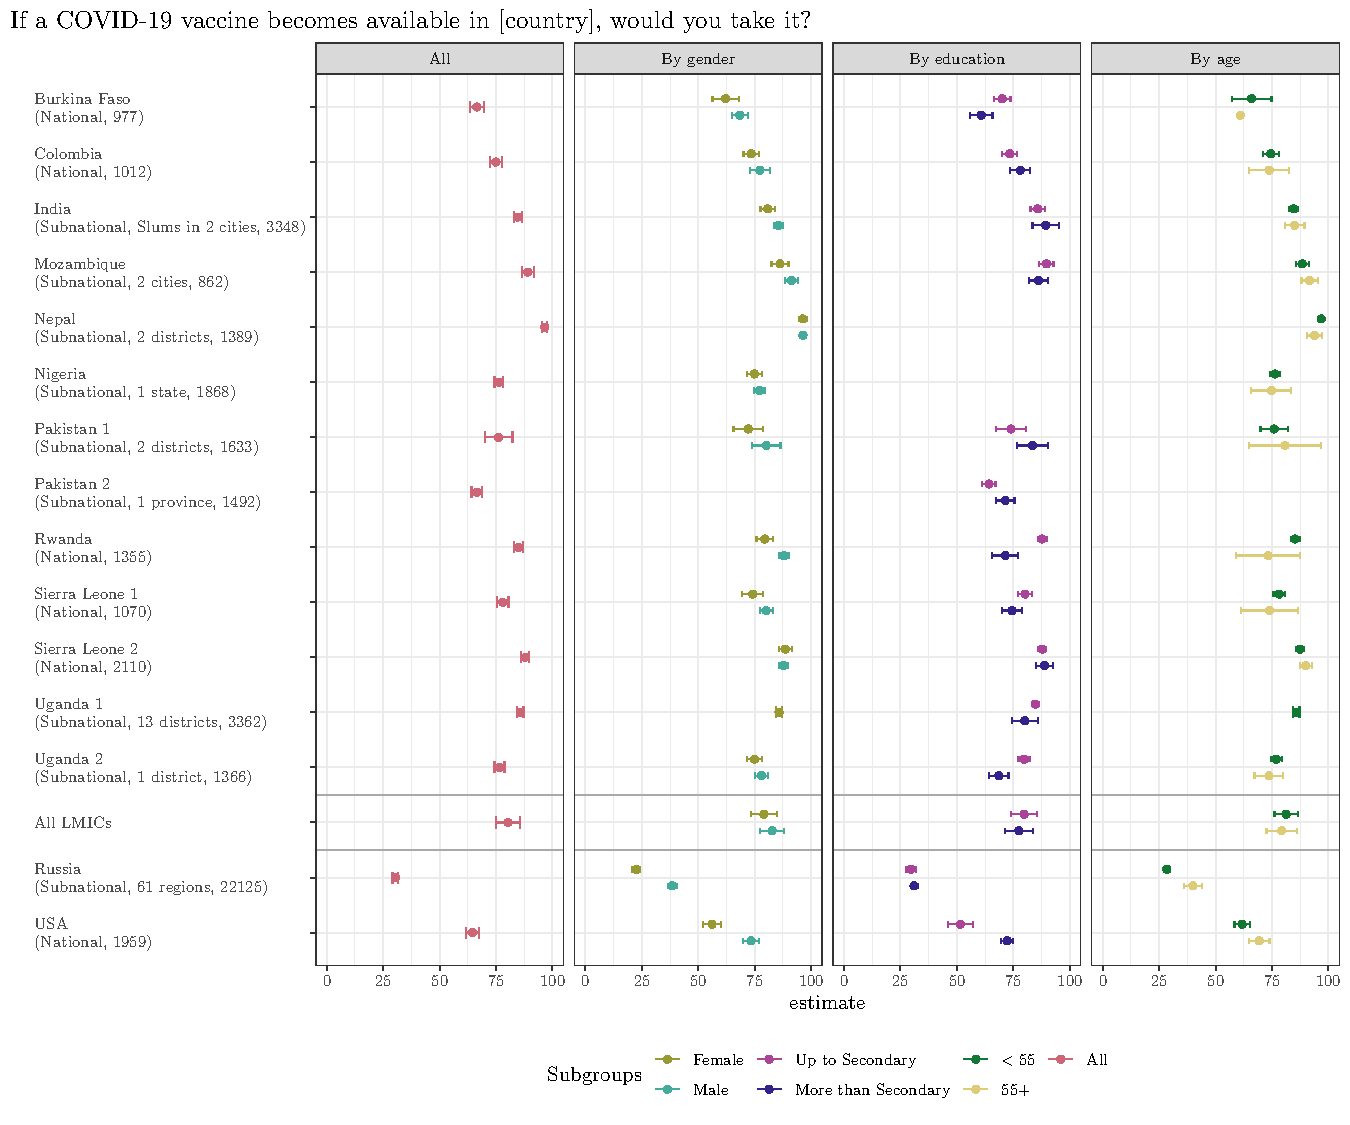
\includegraphics{paper_files/figure-latex/mainfigure1-1.pdf}

\scriptsize{Figure 1 presents average acceptance of the COVID-19 vaccine across studies and subgroups within studies. For each study, we summarize sampling information in parentheses in the following way: First, we indicate whether the geographic coverage of the sample is national or subnational. If the coverage is subnational we provide further details. Second, we list the number of observations included in the study. In the plot, points represent the estimated percentage of individuals who would take the vaccine. ``No'', ``Don't know'' and ``Refuse'' are taken as a single reference category. Bars around each point indicate a 95\% confidence interval for the estimate. An estimate of average acceptance for all studies in LMICs (excluding USA and Russia) is also shown.}
\end{figure}

\begin{Shaded}
\begin{Highlighting}[]
\NormalTok{tab\_reasons\_y}
\end{Highlighting}
\end{Shaded}

\begin{table}

\caption{\label{tab:yes}Reasons to take the vaccine}
\centering
\fontsize{10}{12}\selectfont
\begin{threeparttable}
\begin{tabular}[t]{>{\raggedright\arraybackslash}p{8em}>{\centering\arraybackslash}p{4em}>{\centering\arraybackslash}p{4em}>{\centering\arraybackslash}p{4em}c}
\toprule
\multicolumn{2}{c}{\textbf{ }} & \multicolumn{3}{c}{\textbf{Protection}} \\
\cmidrule(l{3pt}r{3pt}){3-5}
\textbf{Study} & \textbf{N} & \textbf{Self} & \textbf{Family} & \textbf{Community}\\
\midrule
Burkina Faso & 651 & 76 & 42 & 7\\
 &  & (73, 79) & (38, 46) & ( 5,  9)\\
Colombia & 756 & 91 & 23 & 12\\
 &  & (88, 93) & (20, 26) & (10, 14)\\
Mozambique & 768 & 83 & 32 & 4\\
 &  & (80, 86) & (27, 38) & ( 2,  5)\\
Nepal & 1341 & 96 & 34 & 20\\
 &  & (95, 98) & (32, 37) & (17, 22)\\
Nigeria & 1424 & 89 & 35 & 21\\
 &  & (88, 91) & (33, 38) & (19, 23)\\
Rwanda & 1152 & 98 & 26 & 11\\
 &  & (97, 99) & (23, 28) & ( 9, 13)\\
Sierra Leone 1 & 836 & 94 & 37 & 21\\
 &  & (92, 96) & (34, 40) & (18, 23)\\
Sierra Leone 2 & 1855 & 91 & 62 & 21\\
 &  & (88, 93) & (57, 66) & (16, 27)\\
Uganda 1 & 2885 & 96 & 36 & 9\\
 &  & (95, 97) & (34, 38) & ( 8, 10)\\
Uganda 2 & 1045 & 96 & 28 & 11\\
 &  & (95, 97) & (25, 31) & ( 9, 12)\\
All LMICs & . & 91 & 36 & 14\\
 &  & (86, 96) & (28, 43) & ( 9, 18)\\
Russia & 5887 & 76 & 69 & 41\\
 &  & (74, 78) & (67, 71) & (38, 43)\\
USA & 1313 & 94 & 92 & 89\\
 &  & (92, 95) & (90, 94) & (87, 91)\\
\bottomrule
\end{tabular}
\begin{tablenotes}
\item Table 2 shows percentage of respondents mentioning reasons why they would take the Covid-19 vaccine. The number of observations and percentage correponds only to people who would take the vaccine. Respondents in all countries could give more than one reason. A 95\% confidence interval is shown between parentheses. Studies India, Pakistan 1 and Pakistan 2 are not included because they either did not include the question or were not properly harmonized with the other studies.
\end{tablenotes}
\end{threeparttable}
\end{table}

\begin{figure}[!ht]
\caption{Reasons not to take the vaccine \label{fig:fig2paper}}

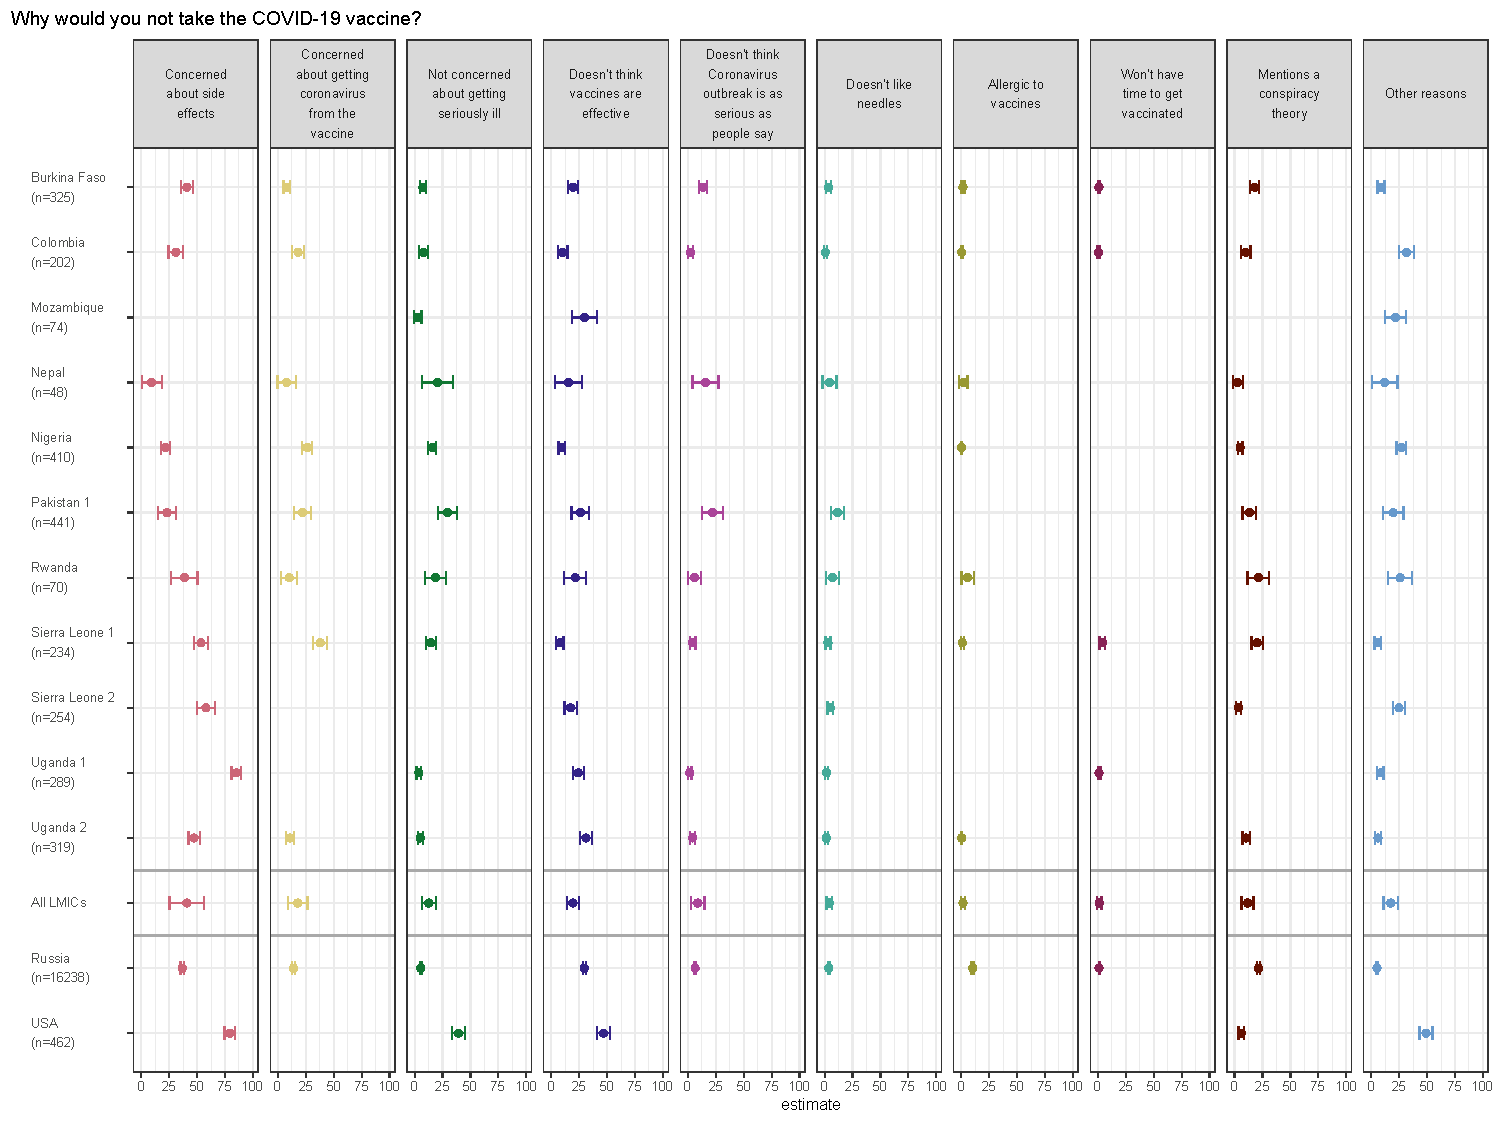
\includegraphics{paper_files/figure-latex/fig2paper-1.pdf}

\scriptsize{Figure 2 shows the percentage of respondents mentioning reasons why they would not take the COVID-19 vaccine. In the plot, points represent the estimated percentage of individuals that would not take the vaccine or do not know if they would take the vaccine for each possible response option. Bars around each point indicate a 95\% confidence interval for the estimate. An estimated average for all studies in LMICs is also shown. Size of points illustrates the number of observations in each response option. Studies India and Pakistan 2 are not included because they either did not include the question or were not properly harmonized with the other studies.}
\end{figure}

\begin{figure}[!ht]
\caption{Trusted actors and institutions, broken down by expressed willingness to take a COVID-19 vaccine \label{fig:fig3paper}}

\newpage

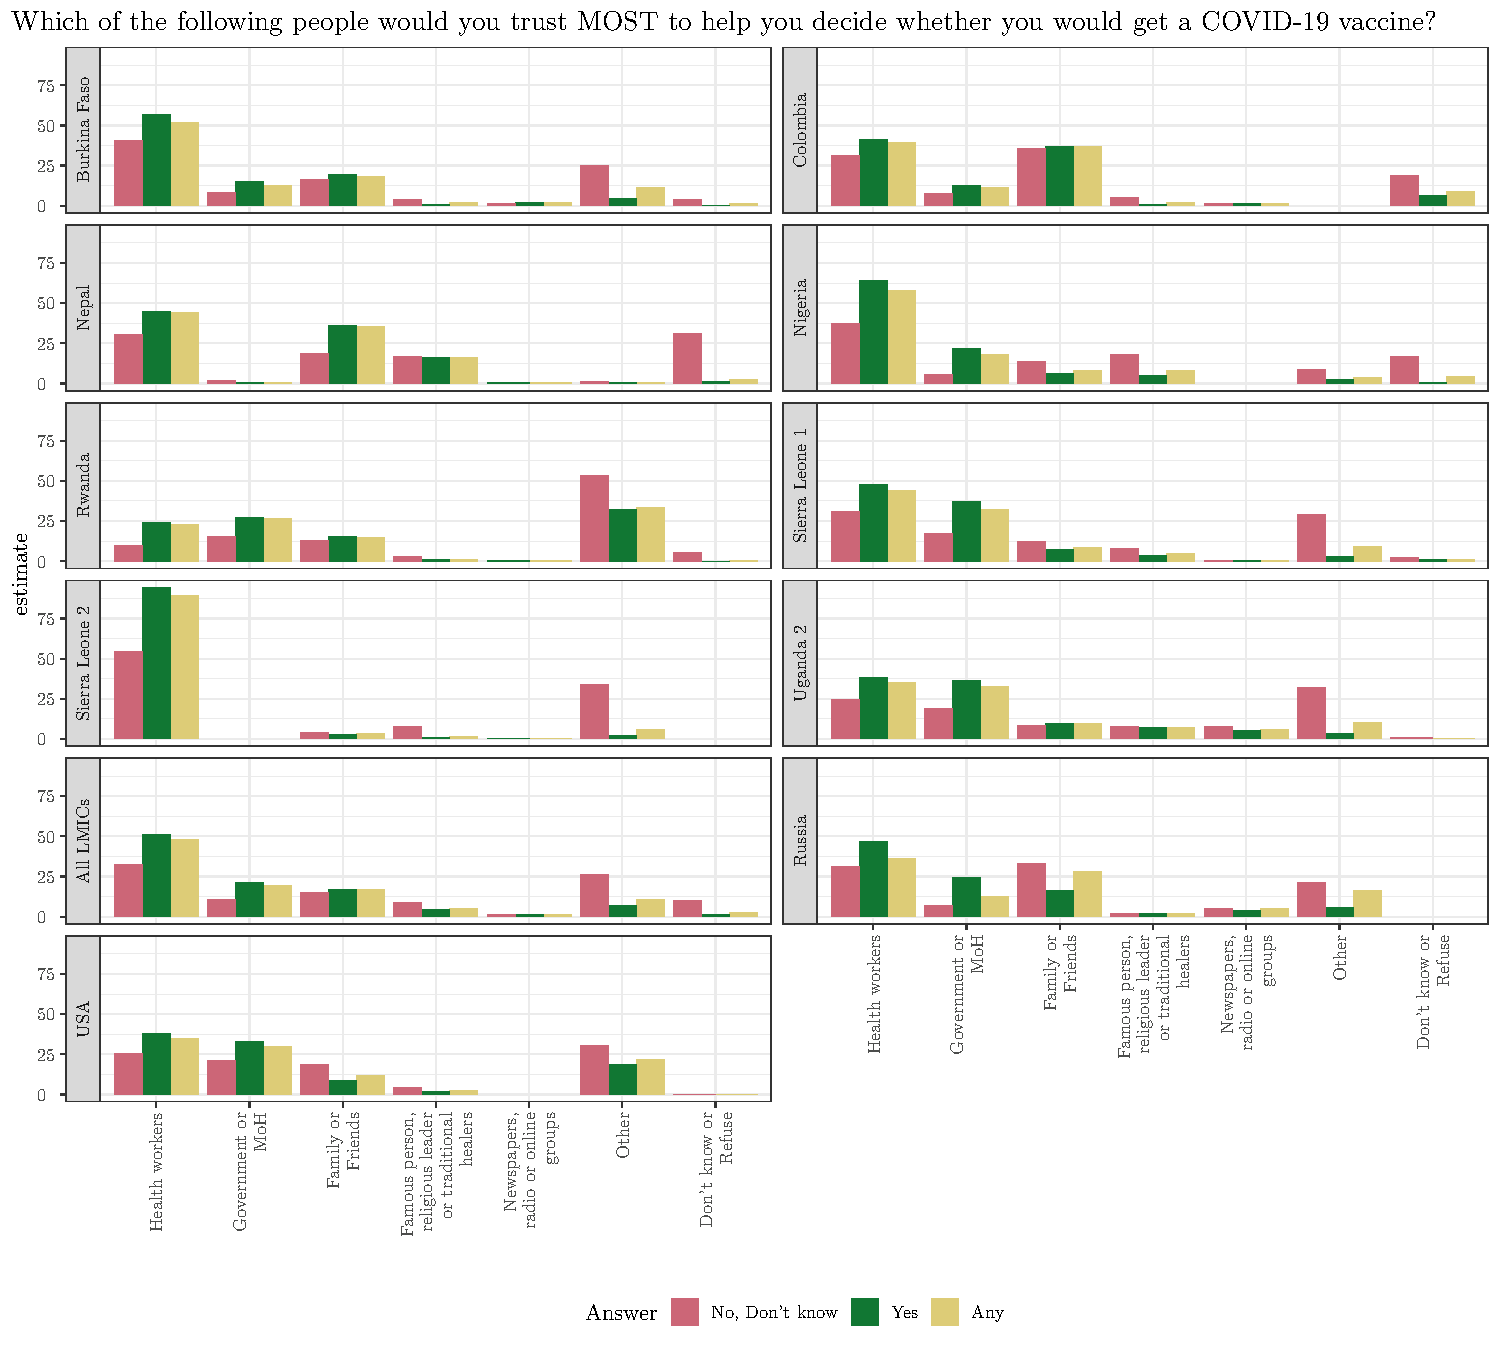
\includegraphics{paper_files/figure-latex/fig3paper-1.pdf}
\newpage

\scriptsize{Figure 3 shows histograms of actors and institutions respondents say they would trust most to help them decide whether to take the COVID-19 vaccine. Respondents were only permitted to select one most trusted actor or institution. Studies India, Mozambique, Pakistan 1, Pakistan 2 and Uganda 1 are not included because they either did not include the question or were not properly harmonized with the other studies.}
\end{figure}

\clearpage

\hypertarget{supplementary-appendix}{%
\section*{Supplementary Appendix}\label{supplementary-appendix}}
\addcontentsline{toc}{section}{Supplementary Appendix}

\hypertarget{appendixd}{%
\subsection*{Appendix A: Supplementary tables, figures and results}\label{appendixd}}
\addcontentsline{toc}{subsection}{Appendix A: Supplementary tables, figures and results}

\begin{Shaded}
\begin{Highlighting}[]
\NormalTok{tab\_sampling}
\end{Highlighting}
\end{Shaded}

\begin{landscape}\begin{table}[!h]

\caption{\label{tab:sampling}Summary of studies sampling}
\centering
\resizebox{\linewidth}{!}{
\fontsize{10}{12}\selectfont
\begin{tabular}[t]{>{\raggedright\arraybackslash}p{8em}>{\raggedright\arraybackslash}p{12em}>{\raggedright\arraybackslash}p{30em}ll}
\toprule
\textbf{Study} & \textbf{Geographic scope} & \textbf{Sampling methodology} & \textbf{Survey modality} & \textbf{Weights}\\
\midrule
Burkina Faso & National & Random digit dialing (RDD) & Phone & Yes\\
Colombia & National & Random digit dialing (RDD) & Phone & Yes\\
India & Subnational, Slums in 2 cities & Representative sample of slum dwellers living in vicinity of a community toilet and located in Uttar Pradesh & Phone & Yes\\
Mozambique & Subnational, 2 cities & 1) Random sample in urban and periurban markets stratified by gender and type of establishment in Maputo; 2) Random sample representative of communities in the Cabo Delgado, stratified on urban, semiurban, and rural areas & Phone & No\\
Nepal & Subnational, 2 districts & Random sample of poor households from randomly selected villages in Kanchanpur & Phone & Yes\\
Nigeria & Subnational, 1 state & 1) Random sample of individuals in Kaduna; 2) Sample of phone numbers from a phone list of Kaduna state residents & Phone & No\\
Pakistan 1 & Subnational, 2 districts & Random sample of individuals in administrative police units in two districts of Punjab & Phone & Yes\\
Pakistan 2 & Subnational, 1 province & Random digit dialing (RDD) on a random sample of all numerically possible mobile phone numbers in the region of Punjab & Phone & No\\
Russia & Subnational, 61 regions & Sample recruited from the Russian online survey company OMI (Online Market Intelligence). Sampling targeted at having a minimum of respondents per region, as well as representation of age, gender and education groups. & Online & Yes\\
Rwanda & National & Random digit dialing (RDD) & Phone & Yes\\
Sierra Leone 1 & National & Random digit dialing (RDD) & Phone & Yes\\
Sierra Leone 2 & National & A random sample of households in 195 rural towns across all 14 districts of Sierra Leone & Phone & No\\
Uganda 1 & Subnational, 13 districts & Sample of women in households from semi-rural and rural villages across 13 districts in Uganda, selected according to the likelihood of having children & Phone & No\\
Uganda 2 & Subnational, 1 district & Random sample of households in Kampala & Phone & No\\
USA & National & Nation-wide sample of adult internet users recruited through the market research firm Lucid & Online & Yes\\
\bottomrule
\end{tabular}}
\end{table}
\end{landscape}

\begin{Shaded}
\begin{Highlighting}[]
\NormalTok{tab\_fig1}
\end{Highlighting}
\end{Shaded}

\begin{table}[!h]

\caption{\label{tab:maintabledis}If a COVID-19 vaccine becomes available in [country], would you take it? Disaggregated by subgroups}
\centering
\resizebox{\linewidth}{!}{
\fontsize{10}{12}\selectfont
\begin{threeparttable}
\begin{tabular}[t]{lccccccc}
\toprule
\multicolumn{1}{c}{\textbf{}} & \multicolumn{1}{c}{\textbf{}} & \multicolumn{2}{c}{\textbf{Gender}} & \multicolumn{2}{c}{\textbf{Education}} & \multicolumn{2}{c}{\textbf{Age}} \\
\cmidrule(l{3pt}r{3pt}){3-4} \cmidrule(l{3pt}r{3pt}){5-6} \cmidrule(l{3pt}r{3pt}){7-8}
\textbf{Country} & \textbf{Average acceptability} & \textbf{Female} & \textbf{Male} & \textbf{> Secondary} & \textbf{Up to Secondary} & \textbf{<55} & \textbf{55+}\\
\midrule
Burkina Faso & 66.5 & 62.1 & 68.4 & 60.8 & 70.1 & 66.0 & 61.0\\
 & (63.5, 69.5) & (56.3, 67.9) & (65.0, 71.9) & (55.9, 65.8) & (66.4, 73.8) & (57.2,  74.8) & (-6.5, 128.6)\\
Colombia & 74.9 & 73.5 & 77.3 & 78.1 & 73.4 & 74.5 & 73.8\\
 & (72.2, 77.6) & (70.1, 77.0) & (73.0, 81.7) & (73.6, 82.5) & (70.1, 76.8) & (70.9,  78.0) & (65.0,  82.6)\\
India & 84.6 & 80.8 & 85.6 & 89.4 & 85.8 & 84.6 & 85.1\\
 & (82.8, 86.4) & (77.6, 84.1) & (83.7, 87.5) & (83.5, 95.4) & (82.6, 88.9) & (82.8,  86.4) & (80.8,  89.4)\\
Mozambique & 89.1 & 86.2 & 91.3 & 86.1 & 89.7 & 88.4 & 91.7\\
 & (86.5, 91.7) & (82.5, 90.0) & (88.4, 94.1) & (81.8, 90.4) & (86.5, 92.8) & (85.5,  91.3) & (88.1,  95.4)\\
Nepal & 96.6 & 96.4 & 96.4 & . & . & 96.8 & 93.8\\
 & (95.5, 97.6) & (94.6, 98.2) & (95.1, 97.7) & . & . & (95.6,  98.0) & (90.4,  97.2)\\
Nigeria & 76.2 & 74.9 & 77.0 & . & . & 76.3 & 74.7\\
 & (74.3, 78.2) & (71.7, 78.1) & (74.6, 79.4) & . & . & (74.3,  78.3) & (65.8,  83.6)\\
Pakistan 1 & 76.1 & 72.2 & 80.1 & 83.6 & 74.0 & 76.0 & 80.8\\
 & (70.0, 82.3) & (65.6, 78.8) & (73.8, 86.4) & (76.6, 90.5) & (67.4, 80.5) & (69.9,  82.2) & (64.9,  96.7)\\
Pakistan 2 & 66.5 & . & . & 71.4 & 64.2 & . & .\\
 & (64.1, 68.9) & . & . & (67.3, 75.5) & (61.2, 67.1) & . & .\\
Rwanda & 84.9 & 79.4 & 88.0 & 71.4 & 87.7 & 85.2 & 73.3\\
 & (82.9, 86.8) & (75.8, 83.0) & (85.8, 90.2) & (65.5, 77.2) & (85.8, 89.7) & (83.3,  87.2) & (59.2,  87.3)\\
Sierra Leone 1 & 78.0 & 74.1 & 80.1 & 74.4 & 80.2 & 78.2 & 74.0\\
 & (75.5, 80.5) & (69.5, 78.7) & (77.2, 83.1) & (70.1, 78.7) & (77.0, 83.3) & (75.7,  80.8) & (61.4,  86.6)\\
Sierra Leone 2 & 87.9 & 88.6 & 87.7 & 88.8 & 87.8 & 87.4 & 90.0\\
 & (86.2, 89.6) & (85.7, 91.5) & (85.9, 89.5) & (85.0, 92.5) & (86.0, 89.6) & (85.5,  89.3) & (87.4,  92.6)\\
Uganda 1 & 85.8 & 85.8 & . & 80.1 & 84.8 & 85.8 & .\\
 & (84.4, 87.2) & (84.4, 87.2) & . & (74.4, 85.9) & (83.2, 86.5) & (84.4,  87.2) & .\\
Uganda 2 & 76.5 & 74.9 & 78.0 & 68.6 & 79.8 & 76.9 & 73.7\\
 & (74.3, 78.7) & (71.5, 78.3) & (75.2, 80.9) & (64.3, 72.9) & (77.3, 82.2) & (74.5,  79.3) & (67.3,  80.0)\\
All LMICs & 80.3 & 79.1 & 82.7 & 77.5 & 79.8 & 81.3 & 79.3\\
 & (74.9, 85.6) & (73.3, 84.9) & (77.4, 88.0) & (71.4, 83.6) & (74.1, 85.4) & (76.1,  86.5) & (72.6,  86.0)\\
Russia & 30.4 & 22.6 & 38.5 & 31.0 & 29.6 & 28.4 & 40.0\\
 & (29.1, 31.7) & (20.9, 24.2) & (36.5, 40.5) & (29.6, 32.5) & (27.3, 32.0) & (27.1,  29.7) & (35.9,  44.0)\\
USA & 64.6 & 56.1 & 73.4 & 72.3 & 51.5 & 61.8 & 69.4\\
 & (61.8, 67.3) & (52.1, 60.1) & (69.8, 76.9) & (69.5, 75.0) & (46.0, 57.0) & (58.4,  65.2) & (64.8,  73.9)\\
\bottomrule
\end{tabular}
\begin{tablenotes}
\item Table 4 shows percentage of respondents willing to take the COVID-19 vaccine as plotted in Figure 1. A 95\% confidence interval is shown between parentheses
\end{tablenotes}
\end{threeparttable}}
\end{table}

\newpage

\begin{Shaded}
\begin{Highlighting}[]
\NormalTok{tab\_reasons\_y\_all}
\end{Highlighting}
\end{Shaded}

\begin{table}[!h]

\caption{\label{tab:yesall}Reasons to take the vaccine- all categories}
\centering
\resizebox{\linewidth}{!}{
\fontsize{10}{12}\selectfont
\begin{threeparttable}
\begin{tabular}[t]{>{\raggedright\arraybackslash}p{7em}>{\centering\arraybackslash}p{7em}>{\centering\arraybackslash}p{7em}>{\centering\arraybackslash}p{7em}>{\centering\arraybackslash}p{7em}>{\centering\arraybackslash}p{7em}>{\centering\arraybackslash}p{7em}>{\centering\arraybackslash}p{7em}}
\toprule
\multicolumn{2}{c}{\textbf{ }} & \multicolumn{3}{c}{\textbf{Protection}} & \multicolumn{2}{c}{\textbf{If recommended by}} & \multicolumn{1}{c}{\textbf{ }} \\
\cmidrule(l{3pt}r{3pt}){3-5} \cmidrule(l{3pt}r{3pt}){6-7}
\textbf{Study} & \textbf{N} & \textbf{Self} & \textbf{Family} & \textbf{Community} & \textbf{Health workers} & \textbf{Government} & \textbf{Other}\\
\midrule
Burkina Faso & 651 & 76 & 42 & 7 & 6 & 19 & 2\\
 &  & (73, 79) & (38, 46) & ( 5,  9) & ( 4,  8) & (16, 22) & ( 1,  3)\\
Colombia & 756 & 91 & 23 & 12 & 1 & 2 & 6\\
 &  & (88, 93) & (20, 26) & (10, 14) & ( 0,  2) & ( 1,  3) & ( 4,  7)\\
Mozambique & 768 & 83 & 32 & 4 & . & 7 & 3\\
 &  & (80, 86) & (27, 38) & ( 2,  5) & . & ( 5,  8) & ( 2,  4)\\
Nepal & 1341 & 96 & 34 & 20 & 2 & 3 & 7\\
 &  & (95, 98) & (32, 37) & (17, 22) & ( 1,  2) & ( 2,  4) & ( 5,  9)\\
Nigeria & 1424 & 89 & 35 & 21 & . & 6 & 4\\
 &  & (88, 91) & (33, 38) & (19, 23) & . & ( 4,  7) & ( 3,  5)\\
Rwanda & 1152 & 98 & 26 & 11 & 1 & 5 & 1\\
 &  & (97, 99) & (23, 28) & ( 9, 13) & ( 0,  1) & ( 4,  6) & ( 1,  2)\\
Sierra Leone 1 & 836 & 94 & 37 & 21 & 12 & 23 & 7\\
 &  & (92, 96) & (34, 40) & (18, 23) & (10, 14) & (20, 25) & ( 5,  9)\\
Sierra Leone 2 & 1855 & 91 & 62 & 21 & 59 & . & 16\\
 &  & (88, 93) & (57, 66) & (16, 27) & (54, 63) & . & (11, 21)\\
Uganda 1 & 2885 & 96 & 36 & 9 & . & 10 & 6\\
 &  & (95, 97) & (34, 38) & ( 8, 10) & . & ( 9, 12) & ( 5,  7)\\
Uganda 2 & 1045 & 96 & 28 & 11 & 1 & 15 & 2\\
 &  & (95, 97) & (25, 31) & ( 9, 12) & ( 1,  2) & (13, 17) & ( 1,  3)\\
All LMICs & . & 91 & 36 & 14 & 12 & 10 & 5\\
 &  & (86, 96) & (28, 43) & ( 9, 18) & (-8, 31) & ( 4, 16) & ( 2,  8)\\
Russia & 5887 & 76 & 69 & 41 & 11 & 6 & 18\\
 &  & (74, 78) & (67, 71) & (38, 43) & (10, 13) & ( 5,  7) & (16, 20)\\
USA & 1313 & 94 & 92 & 89 & . & 67 & .\\
 &  & (92, 95) & (90, 94) & (87, 91) & . & (64, 70) & .\\
\bottomrule
\end{tabular}
\begin{tablenotes}
\item Table 5 shows percentage of respondents mentioning reasons why they would take the Covid-19 vaccine. The number of observations and percentage correponds only to people who would take the vaccine. Respondents in all countries could give more than one reason. A 95\% confidence interval is shown between parentheses
\end{tablenotes}
\end{threeparttable}}
\end{table}

\newpage

\begin{Shaded}
\begin{Highlighting}[]
\NormalTok{tab\_fig2}
\end{Highlighting}
\end{Shaded}

\begin{landscape}\begin{table}[!h]

\caption{\label{tab:no}Reasons not to take the vaccine}
\centering
\resizebox{\linewidth}{!}{
\fontsize{10}{12}\selectfont
\begin{threeparttable}
\begin{tabular}[t]{>{\raggedright\arraybackslash}p{7em}>{\centering\arraybackslash}p{7em}>{\centering\arraybackslash}p{7em}>{\centering\arraybackslash}p{7em}>{\centering\arraybackslash}p{7em}>{\centering\arraybackslash}p{7em}>{\centering\arraybackslash}p{7em}>{\centering\arraybackslash}p{7em}>{\centering\arraybackslash}p{7em}>{\centering\arraybackslash}p{7em}>{\centering\arraybackslash}p{7em}>{\centering\arraybackslash}p{7em}}
\toprule
\textbf{Study} & \textbf{N} & \textbf{Concerned about side effects} & \textbf{Concerned about getting coronavirus from the vaccine} & \textbf{Not concerned about getting seriously ill} & \textbf{Doesn't think vaccines are effective} & \textbf{Doesn't think Coronavirus outbreak is as serious as people say} & \textbf{Doesn't like needles} & \textbf{Allergic to vaccines} & \textbf{Won't have time to get vaccinated} & \textbf{Mentions a conspiracy theory} & \textbf{Other reasons}\\
\midrule
Burkina Faso & 325 & 40.9 & 8.0 & 7.4 & 19.5 & 13.5 & 3.5 & 1.5 & 0.9 & 17.9 & 8.7\\
 &  & (35.5, 46.3) & ( 5.0, 11.0) & ( 4.5, 10.2) & (15.1, 23.8) & ( 9.8, 17.2) & ( 1.5,  5.6) & ( 0.2,  2.8) & (-0.1,  1.9) & (13.7, 22.1) & ( 5.6, 11.8)\\
Colombia & 202 & 31.0 & 18.1 & 8.0 & 10.2 & 2.3 & 0.6 & 0.4 & 0.5 & 10.0 & 31.6\\
 &  & (24.4, 37.6) & (12.7, 23.4) & ( 3.9, 12.0) & ( 5.9, 14.5) & ( 0.3,  4.3) & (-0.6,  1.8) & (-0.4,  1.3) & (-0.5,  1.5) & ( 5.8, 14.2) & (25.1, 38.2)\\
Mozambique & 74 & . & . & 2.7 & 29.7 & . & . & . & . & . & 21.6\\
 &  & . & . & (-0.7,  6.1) & (18.6, 40.8) & . & . & . & . & . & (12.2, 31.0)\\
Nepal & 48 & 9.3 & 7.9 & 20.4 & 15.2 & 15.7 & 4.4 & 1.8 & . & 2.8 & 12.1\\
 &  & ( 0.3, 18.2) & (-0.4, 16.3) & ( 6.7, 34.1) & ( 3.2, 27.2) & ( 4.0, 27.3) & (-1.9, 10.6) & (-1.9,  5.5) & . & (-1.5,  7.2) & ( 0.8, 23.5)\\
Nigeria & 410 & 21.5 & 26.1 & 15.9 & 9.3 & . & . & 0.2 & . & 4.9 & 26.8\\
 &  & (17.5, 25.5) & (21.8, 30.4) & (12.3, 19.4) & ( 6.4, 12.1) & . & . & (-0.2,  0.7) & . & ( 2.8,  7.0) & (22.5, 31.1)\\
Pakistan 1 & 441 & 23.0 & 21.9 & 29.4 & 26.0 & 22.1 & 11.5 & . & . & 13.2 & 19.6\\
 &  & (15.1, 30.8) & (14.3, 29.4) & (20.9, 37.9) & (18.0, 34.0) & (12.8, 31.3) & ( 5.5, 17.4) & . & . & ( 7.1, 19.4) & (10.4, 28.8)\\
Rwanda & 70 & 38.6 & 10.1 & 18.7 & 21.5 & 5.8 & 7.0 & 5.6 & . & 21.3 & 25.8\\
 &  & (26.9, 50.3) & ( 2.8, 17.3) & ( 9.3, 28.1) & (11.6, 31.4) & ( 0.1, 11.4) & ( 0.9, 13.2) & ( 0.1, 11.1) & . & (11.5, 31.1) & (15.3, 36.3)\\
Sierra Leone 1 & 234 & 53.5 & 37.9 & 14.6 & 7.5 & 4.2 & 3.0 & 0.9 & 4.0 & 20.3 & 5.7\\
 &  & (47.1, 59.9) & (31.6, 44.2) & (10.1, 19.2) & ( 4.2, 10.9) & ( 1.6,  6.8) & ( 0.8,  5.2) & (-0.4,  2.2) & ( 1.4,  6.5) & (15.1, 25.5) & ( 2.8,  8.7)\\
Sierra Leone 2 & 254 & 57.9 & . & . & 17.3 & . & 5.1 & . & 0.0 & 3.5 & 24.8\\
 &  & (50.1, 65.7) & . & . & (11.9, 22.7) & . & ( 2.5,  7.8) & . & ( 0.0,  0.0) & ( 1.3,  5.7) & (19.3, 30.3)\\
Uganda 1 & 289 & 85.1 & . & 3.8 & 24.2 & 1.7 & 1.7 & . & 1.0 & . & 8.0\\
 &  & (80.7, 89.6) & . & ( 1.7,  5.9) & (19.2, 29.2) & ( 0.2,  3.2) & ( 0.2,  3.2) & . & (-0.1,  2.2) & . & ( 4.9, 11.0)\\
Uganda 2 & 319 & 47.3 & 10.7 & 5.0 & 31.0 & 4.1 & 1.6 & 0.3 & . & 10.3 & 6.0\\
 &  & (42.2, 52.5) & ( 7.1, 14.2) & ( 2.7,  7.3) & (25.9, 36.2) & ( 1.9,  6.2) & ( 0.2,  2.9) & (-0.3,  0.9) & . & ( 7.0, 13.7) & ( 3.4,  8.5)\\
All LMICs & . & 40.8 & 17.6 & 12.6 & 19.2 & 8.7 & 4.3 & 1.5 & 1.3 & 11.6 & 17.3\\
 &  & (25.3, 56.3) & ( 8.7, 26.5) & ( 6.4, 18.8) & (13.8, 24.7) & ( 2.4, 14.9) & ( 1.7,  6.8) & (-0.2,  3.3) & (-0.6,  3.2) & ( 6.1, 17.0) & (11.0, 23.7)\\
Russia & 16238 & 36.8 & 13.9 & 5.4 & 29.6 & 6.4 & 3.7 & 10.2 & 1.0 & 21.4 & 5.1\\
 &  & (35.2, 38.4) & (12.8, 15.1) & ( 4.6,  6.1) & (28.1, 31.1) & ( 5.6,  7.3) & ( 3.1,  4.3) & ( 9.2, 11.2) & ( 0.7,  1.4) & (20.1, 22.8) & ( 4.4,  5.8)\\
USA & 462 & 79.3 & . & 39.3 & 46.8 & . & . & . & . & 6.0 & 49.1\\
 &  & (74.6, 84.0) & . & (33.5, 45.0) & (41.0, 52.6) & . & . & . & . & ( 3.4,  8.7) & (43.3, 54.9)\\
\bottomrule
\end{tabular}
\begin{tablenotes}
\item Table 6 shows percentage of respondents mentioning reasons why they would not take the Covid-19 vaccine. The number of observations and percentage correponds only to people who would NOT take the vaccine. Respondents in all countries could give more than one reason. A 95\% confidence interval is shown between parentheses
\end{tablenotes}
\end{threeparttable}}
\end{table}
\end{landscape}

\newpage

\begin{Shaded}
\begin{Highlighting}[]
\NormalTok{tab\_trust}
\end{Highlighting}
\end{Shaded}

\begin{landscape}\begingroup\fontsize{10}{12}\selectfont

\begin{ThreePartTable}
\begin{TableNotes}
\item Table 7 shows percentage of respondents that mention actors who they would trust the most to help them decide whether to get a COVID-19 vaccine. For all countries the questions was asked regardless if respondent would take a vaccine, would not take it, does not know or does not respond. For India respondents were able to mention more than one actor, for the rest of countries only one actor was allowed. While rows should sum to 100\%, rounding makes number slightly above or below. A 95\% confidence interval is shown between parentheses.
\end{TableNotes}
\begin{longtable}[t]{>{\raggedright\arraybackslash}p{7em}>{\centering\arraybackslash}p{4em}>{\centering\arraybackslash}p{4em}>{\centering\arraybackslash}p{6em}>{\centering\arraybackslash}p{6em}>{\centering\arraybackslash}p{6em}>{\centering\arraybackslash}p{6em}>{\centering\arraybackslash}p{6em}>{\centering\arraybackslash}p{6em}>{\centering\arraybackslash}p{6em}}
\caption{\label{tab:trust}COVID-19 Vaccination Decision-making: most trusted source}\\
\toprule
\textbf{Study} & \textbf{N} & \textbf{Take vaccine?} & \textbf{Health workers} & \textbf{Government or Ministry of Health} & \textbf{Family or friends} & \textbf{Famous person, religious leader or traditional healers} & \textbf{Newspapers, radio or online groups} & \textbf{Other} & \textbf{Don't know or Refuse}\\
\midrule
\endfirsthead
\caption[]{\label{tab:trust}COVID-19 Vaccination Decision-making: most trusted source \textit{(continued)}}\\
\toprule
\textbf{Study} & \textbf{N} & \textbf{Take vaccine?} & \textbf{Health workers} & \textbf{Government or Ministry of Health} & \textbf{Family or friends} & \textbf{Famous person, religious leader or traditional healers} & \textbf{Newspapers, radio or online groups} & \textbf{Other} & \textbf{Don't know or Refuse}\\
\midrule
\endhead

\endfoot
\bottomrule
\insertTableNotes
\endlastfoot
Burkina Faso & 651 & Yes & 57.1 & 15.1 & 19.6 & 0.9 & 2.0 & 4.8 & 0.4\\
 &  &  & (53.3, 60.9) & (12.4, 17.9) & (16.5, 22.7) & ( 0.2,  1.6) & ( 0.9,  3.1) & ( 3.2,  6.4) & (-0.1,  0.9)\\
Burkina Faso & 325 & No & 40.7 & 8.5 & 16.2 & 3.7 & 1.6 & 25.1 & 4.2\\
 &  &  & (35.3, 46.1) & ( 5.5, 11.6) & (12.1, 20.2) & ( 1.6,  5.7) & ( 0.2,  3.0) & (20.3, 29.8) & ( 2.0,  6.4)\\
Burkina Faso & 976 & All & 51.6 & 12.9 & 18.4 & 1.8 & 1.9 & 11.6 & 1.7\\
 &  &  & (48.5, 54.8) & (10.8, 15.0) & (16.0, 20.9) & ( 1.0,  2.7) & ( 1.0,  2.7) & ( 9.6, 13.6) & ( 0.9,  2.5)\\
Colombia & 756 & Yes & 41.4 & 12.7 & 36.9 & 0.9 & 1.7 & . & 6.3\\
 &  &  & (37.8, 45.0) & (10.3, 15.2) & (33.4, 40.4) & ( 0.2,  1.5) & ( 0.8,  2.7) & . & ( 4.6,  8.1)\\
Colombia & 202 & No & 31.5 & 7.6 & 35.5 & 5.3 & 1.4 & . & 18.8\\
 &  &  & (24.9, 38.1) & ( 3.8, 11.3) & (28.8, 42.1) & ( 2.2,  8.4) & (-0.2,  3.0) & . & (13.2, 24.3)\\
Colombia & 958 & All & 39.3 & 11.6 & 36.6 & 1.8 & 1.7 & . & 8.9\\
 &  &  & (36.2, 42.5) & ( 9.6, 13.7) & (33.5, 39.7) & ( 1.0,  2.6) & ( 0.9,  2.5) & . & ( 7.1, 10.7)\\
Nepal & 1341 & Yes & 44.7 & 0.7 & 36.2 & 16.1 & 0.4 & 0.5 & 1.3\\
 &  &  & (40.9, 48.6) & ( 0.3,  1.1) & (33.5, 39.0) & (13.1, 19.1) & ( 0.0,  0.9) & ( 0.1,  0.8) & ( 0.7,  2.0)\\
Nepal & 48 & No & 30.2 & 2.1 & 18.7 & 16.8 & 0.0 & 1.0 & 31.2\\
 &  &  & (14.6, 45.9) & (-2.1,  6.2) & ( 5.6, 31.7) & ( 4.0, 29.6) & ( 0.0,  0.0) & (-1.1,  3.2) & (13.6, 48.9)\\
Nepal & 1389 & All & 44.2 & 0.8 & 35.6 & 16.1 & 0.4 & 0.5 & 2.4\\
 &  &  & (40.5, 47.9) & ( 0.3,  1.2) & (32.9, 38.3) & (13.3, 18.9) & ( 0.0,  0.8) & ( 0.1,  0.8) & ( 1.5,  3.3)\\
Nigeria & 1424 & Yes & 63.8 & 21.6 & 6.3 & 5.1 & . & 2.6 & 0.6\\
 &  &  & (61.3, 66.3) & (19.4, 23.7) & ( 5.0,  7.5) & ( 4.0,  6.3) & . & ( 1.8,  3.4) & ( 0.2,  1.0)\\
Nigeria & 410 & No & 37.6 & 5.6 & 13.9 & 17.8 & . & 8.5 & 16.6\\
 &  &  & (32.9, 42.3) & ( 3.4,  7.8) & (10.5, 17.3) & (14.1, 21.5) & . & ( 5.8, 11.3) & (13.0, 20.2)\\
Nigeria & 1834 & All & 58.0 & 18.0 & 8.0 & 8.0 & . & 3.9 & 4.2\\
 &  &  & (55.7, 60.2) & (16.2, 19.8) & ( 6.7,  9.2) & ( 6.7,  9.2) & . & ( 3.0,  4.8) & ( 3.3,  5.1)\\
Rwanda & 1152 & Yes & 23.8 & 27.4 & 15.1 & 1.0 & 0.7 & 32.0 & 0.1\\
 &  &  & (21.3, 26.2) & (24.9, 30.0) & (13.0, 17.2) & ( 0.4,  1.5) & ( 0.2,  1.2) & (29.3, 34.7) & (-0.1,  0.2)\\
Rwanda & 70 & No & 10.1 & 15.6 & 12.8 & 2.9 & 0.0 & 53.2 & 5.5\\
 &  &  & ( 2.8, 17.4) & ( 6.9, 24.3) & ( 4.8, 20.8) & (-1.1,  6.9) & ( 0.0,  0.0) & (41.2, 65.1) & ( 0.1, 11.0)\\
Rwanda & 1222 & All & 23.0 & 26.7 & 15.0 & 1.1 & 0.6 & 33.2 & 0.4\\
 &  &  & (20.6, 25.3) & (24.3, 29.2) & (13.0, 17.0) & ( 0.5,  1.7) & ( 0.2,  1.1) & (30.5, 35.8) & ( 0.0,  0.8)\\
Sierra Leone 1 & 836 & Yes & 47.6 & 36.9 & 7.3 & 3.8 & 0.5 & 3.1 & 0.8\\
 &  &  & (44.2, 51.0) & (33.6, 40.2) & ( 5.5,  9.1) & ( 2.5,  5.1) & ( 0.0,  1.0) & ( 1.9,  4.2) & ( 0.2,  1.4)\\
Sierra Leone 1 & 234 & No & 31.1 & 17.1 & 12.1 & 7.7 & 0.5 & 29.4 & 2.2\\
 &  &  & (25.1, 37.1) & (12.2, 21.9) & ( 7.9, 16.3) & ( 4.3, 11.2) & (-0.4,  1.3) & (23.5, 35.3) & ( 0.3,  4.1)\\
Sierra Leone 1 & 1070 & All & 44.0 & 32.5 & 8.4 & 4.7 & 0.5 & 8.9 & 1.1\\
 &  &  & (41.0, 46.9) & (29.7, 35.4) & ( 6.7, 10.0) & ( 3.4,  6.0) & ( 0.1,  0.9) & ( 7.1, 10.6) & ( 0.5,  1.8)\\
Sierra Leone 2 & 1855 & Yes & 94.1 & . & 3.0 & 0.9 & 0.1 & 1.9 & 0.0\\
 &  &  & (92.5, 95.7) & . & ( 2.0,  4.0) & ( 0.3,  1.5) & (-0.1,  0.2) & ( 1.2,  2.7) & ( 0.0,  0.0)\\
Sierra Leone 2 & 254 & No & 54.7 & . & 3.9 & 7.5 & 0.0 & 33.9 & 0.0\\
 &  &  & (46.5, 62.9) & . & ( 1.4,  6.5) & ( 2.9, 12.0) & ( 0.0,  0.0) & (26.3, 41.4) & ( 0.0,  0.0)\\
Sierra Leone 2 & 2109 & All & 89.3 & . & 3.1 & 1.7 & 0.0 & 5.8 & 0.0\\
 &  &  & (87.2, 91.5) & . & ( 2.2,  4.1) & ( 0.8,  2.6) & ( 0.0,  0.1) & ( 4.4,  7.2) & ( 0.0,  0.0)\\
Uganda 2 & 1045 & Yes & 38.3 & 36.5 & 9.8 & 7.0 & 5.0 & 3.5 & 0.0\\
 &  &  & (35.5, 41.1) & (33.5, 39.4) & ( 7.9, 11.6) & ( 5.4,  8.6) & ( 3.6,  6.3) & ( 2.5,  4.6) & ( 0.0,  0.0)\\
Uganda 2 & 319 & No & 24.5 & 19.1 & 8.5 & 7.8 & 7.5 & 32.0 & 0.6\\
 &  &  & (19.9, 29.0) & (14.5, 23.7) & ( 5.4, 11.5) & ( 4.8, 10.9) & ( 4.5, 10.5) & (26.7, 37.3) & (-0.2,  1.5)\\
Uganda 2 & 1364 & All & 35.0 & 32.4 & 9.5 & 7.2 & 5.6 & 10.2 & 0.1\\
 &  &  & (32.7, 37.4) & (29.9, 35.0) & ( 7.9, 11.1) & ( 5.8,  8.6) & ( 4.3,  6.8) & ( 8.6, 11.8) & (-0.1,  0.3)\\
All LMICs & . & Yes & 51.3 & 21.6 & 16.8 & 4.5 & 1.5 & 6.9 & 1.2\\
 &  &  & (33.7, 68.9) & ( 9.4, 33.8) & ( 5.7, 27.9) & ( 0.1,  8.8) & (-0.1,  3.1) & (-3.4, 17.2) & (-0.6,  3.0)\\
All LMICs & . & No & 32.5 & 10.8 & 15.2 & 8.7 & 1.6 & 26.1 & 9.9\\
 &  &  & (21.8, 43.3) & ( 4.8, 16.8) & ( 7.4, 23.0) & ( 4.0, 13.4) & (-0.9,  4.1) & (10.2, 42.1) & ( 0.6, 19.2)\\
All LMICs & . & All & 48.1 & 19.3 & 16.8 & 5.3 & 1.5 & 10.6 & 2.4\\
 &  &  & (31.6, 64.5) & ( 8.3, 30.3) & ( 6.1, 27.5) & ( 1.0,  9.6) & (-0.2,  3.3) & ( 0.7, 20.5) & (-0.1,  4.9)\\
Russia & 5887 & Yes & 47.1 & 24.4 & 16.5 & 2.0 & 4.1 & 5.8 & .\\
 &  &  & (44.6, 49.7) & (22.2, 26.7) & (14.6, 18.5) & ( 1.2,  2.8) & ( 3.1,  5.1) & ( 4.5,  7.0) & .\\
Russia & 16238 & No & 31.1 & 6.9 & 33.1 & 2.2 & 5.3 & 21.3 & .\\
 &  &  & (29.6, 32.7) & ( 6.1,  7.8) & (31.5, 34.7) & ( 1.7,  2.8) & ( 4.5,  6.0) & (20.0, 22.7) & .\\
Russia & 22125 & All & 36.0 & 12.3 & 28.1 & 2.2 & 4.9 & 16.6 & .\\
 &  &  & (34.7, 37.3) & (11.3, 13.2) & (26.8, 29.3) & ( 1.7,  2.6) & ( 4.3,  5.5) & (15.6, 17.6) & .\\
USA & 1313 & Yes & 38.1 & 33.0 & 8.7 & 1.7 & . & 18.6 & 0.0\\
 &  &  & (34.8, 41.5) & (29.8, 36.1) & ( 6.7, 10.7) & ( 0.7,  2.6) & . & (16.1, 21.1) & ( 0.0,  0.0)\\
USA & 462 & No & 25.3 & 21.3 & 18.7 & 4.2 & . & 30.3 & 0.2\\
 &  &  & (20.4, 30.3) & (16.6, 26.0) & (13.9, 23.4) & ( 1.6,  6.9) & . & (25.0, 35.6) & (-0.2,  0.7)\\
USA & 1775 & All & 34.5 & 29.7 & 11.5 & 2.4 & . & 21.9 & 0.1\\
 &  &  & (31.7, 37.3) & (27.0, 32.3) & ( 9.5, 13.4) & ( 1.4,  3.4) & . & (19.5, 24.2) & (-0.1,  0.2)\\*
\end{longtable}
\end{ThreePartTable}
\endgroup{}
\end{landscape}
\newpage

\begin{figure}[!ht]
\caption{Trusted actors and institutions, broken down by gender \label{fig:genderhist}}

\begin{Shaded}
\begin{Highlighting}[]
\NormalTok{hist\_gender}
\end{Highlighting}
\end{Shaded}

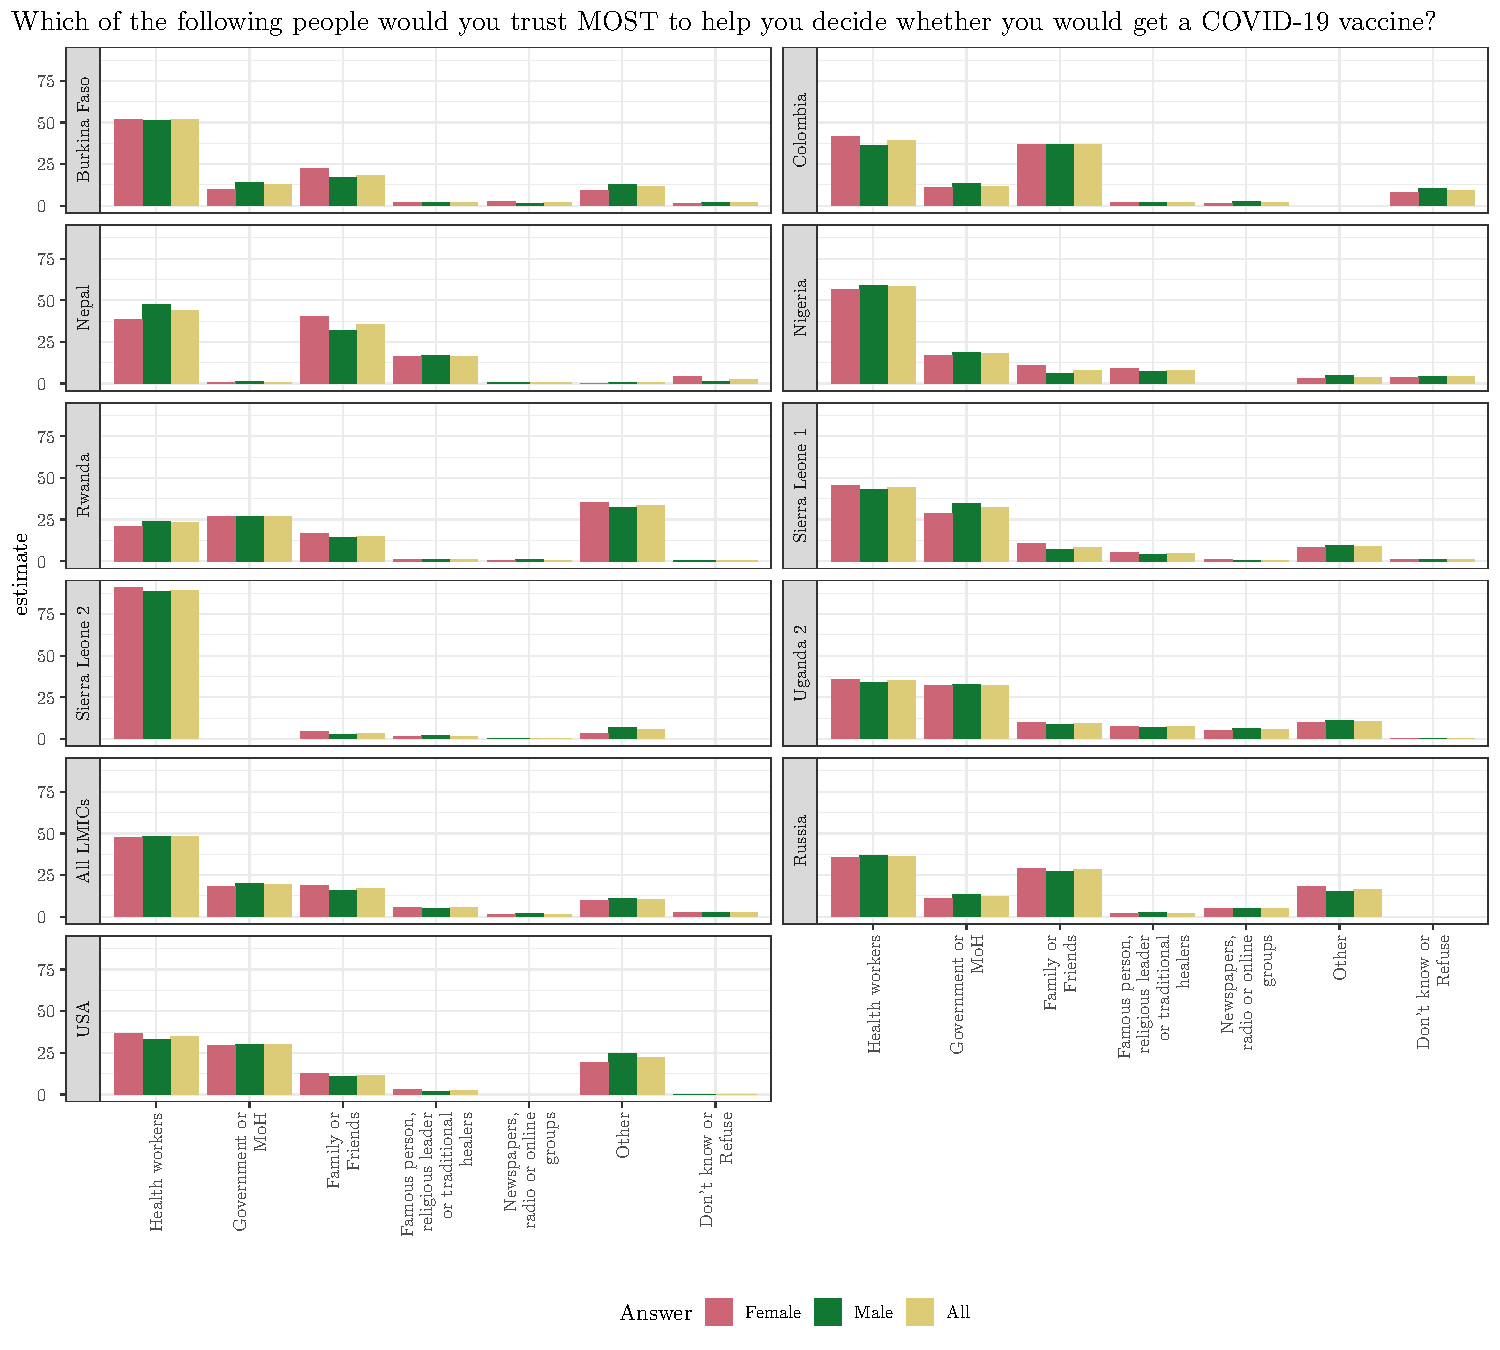
\includegraphics{paper_files/figure-latex/genderhist-1.pdf}

\scriptsize{Figure 4 shows histograms of actors and institutions that respondents say they would trust most to help them decide whether or not to take the COVID-19 vaccine. Respondents were only permitted to select one most trusted  actor or institution. Responses are broken down by acceptance of the COVID-19 vaccine.}
\end{figure}

\pagebreak

\begin{Shaded}
\begin{Highlighting}[]
\NormalTok{dmeans}
\end{Highlighting}
\end{Shaded}

\begin{table}[!h]

\caption{\label{tab:dmeans}Differences in means}
\centering
\fontsize{10}{12}\selectfont
\begin{threeparttable}
\begin{tabular}[t]{cccccc}
\toprule
\textbf{Estimate} & \textbf{Std.error} & \textbf{P.value} & \textbf{Degrees of freedom} & \textbf{Baseline category} & \textbf{Variable}\\
\midrule
0.04 & 0.01 & 0.00 & 10 & Male & Gender\\
0.00 & 0.01 & 0.71 & 10 & 55+ & Age\\
0.02 & 0.03 & 0.41 & 10 & Up to secondary & Education\\
\bottomrule
\end{tabular}
\begin{tablenotes}
\item Table 8 shows the results of subgroup mean differences. Subgroup differences were generated considering only LMICs. The differences in means for gender and age do not include the Uganda 1 study, which only included female respondents under the age of 55. p-values come from a two-sided t-test from a linear regression.
\end{tablenotes}
\end{threeparttable}
\end{table}

\clearpage

\begin{Shaded}
\begin{Highlighting}[]
\NormalTok{nas}
\end{Highlighting}
\end{Shaded}

\begin{table}

\caption{Observations and missingness patterns}
\centering
\fontsize{10}{12}\selectfont
\begin{threeparttable}
\begin{tabular}[t]{lrrrrr}
\toprule
Country & N obs & Take vaccine & Gender & Education & Age\\
\midrule
Burkina Faso & 977 & 1.00 & 0.00 & 0.00 & 0.88\\
Colombia & 1,012 & 0.95 & 0.00 & 0.00 & 0.32\\
India & 3,348 & 1.00 & 0.00 & 0.78 & 0.00\\
Mozambique & 862 & 0.98 & 0.00 & 0.04 & 0.00\\
Nepal & 1,389 & 1.00 & 0.05 & 1.00 & 0.05\\
Nigeria & 1,868 & 0.98 & 0.00 & 1.00 & 0.00\\
Pakistan 1 & 1,633 & 0.99 & 0.00 & 0.01 & 0.00\\
Pakistan 2 & 1,492 & 1.00 & 1.00 & 0.00 & 1.00\\
Russia & 22,125 & 1.00 & 0.00 & 0.00 & 0.00\\
Rwanda & 1,355 & 0.90 & 0.00 & 0.00 & 0.00\\
Sierra Leone 1 & 1,070 & 1.00 & 0.00 & 0.03 & 0.00\\
Sierra Leone 2 & 2,110 & 1.00 & 0.00 & 0.00 & 0.01\\
Uganda 1 & 3,362 & 0.94 & 0.00 & 0.19 & 0.05\\
Uganda 2 & 1,366 & 1.00 & 0.00 & 0.00 & 0.00\\
USA & 1,959 & 0.91 & 0.00 & 0.00 & 0.00\\
\bottomrule
\end{tabular}
\begin{tablenotes}
\item Table 9 show the percentage of observations that are not missing values for each variable included in Figure 1.
\end{tablenotes}
\end{threeparttable}
\end{table}

\begin{center}\rule{0.5\linewidth}{0.5pt}\end{center}

\pagebreak

\hypertarget{appendixb}{%
\subsection*{Appendix B: Question wording and answer options per study}\label{appendixb}}
\addcontentsline{toc}{subsection}{Appendix B: Question wording and answer options per study}

\begin{Shaded}
\begin{Highlighting}[]
\NormalTok{tab\_question1}
\end{Highlighting}
\end{Shaded}

\begin{table}[!h]

\caption{\label{tab:q1}Question wording and answer options: vaccine acceptance}
\centering
\resizebox{\linewidth}{!}{
\fontsize{10}{12}\selectfont
\begin{threeparttable}
\begin{tabular}[t]{>{\raggedright\arraybackslash}p{8em}>{\raggedright\arraybackslash}p{30em}>{\raggedright\arraybackslash}p{20em}}
\toprule
\textbf{Study} & \textbf{Question Fig. 1} & \textbf{Recoding Fig. 1}\\
\midrule
Burkina Faso & If a COVID-19 vaccine became available in Burkina Faso, would you take it? & Yes; No; Don't know; Refuse\\
Colombia & If a COVID-19 vaccine became available in Colombia, would you take it? & Yes; No\\
India & If a vaccine for coronavirus gets introduced, would you like to get it? & Yes, only for free; Yes, even if I have to pay; No\\
Mozambique & When a COVID-19 vaccine becomes available in the future, would you take it? & Yes; No; Refuse\\
Nepal & Should a vaccine against COVID become available in Nepal, would you take it? & Yes; No\\
Nigeria & If a COVID-19 vaccine became available in Niger, would you take it? & Yes/Agree; No/Disagree\\
Pakistan 1 & If a vaccine against the coronavirus becomes available, do you plan to get vaccinated? & Yes; No; Don't know; Refuse\\
Pakistan 2 & If a vaccine against the coronavirus becomes available, do you plan to get vaccinated? & Absolutely yes; Yes; Neutral; No; Absolutely no\\
Russia & If a COVID-19 vaccine became available in Russia, would you take it? & Yes, if a Russian vaccine will be available; Yes, if an imported vaccine will be available; No; Not sure\\
Rwanda & If a COVID-19 vaccine became available in Rwanda, would you take it? & Yes; No\\
Sierra Leone 1 & If a COVID-19 vaccine became available in Sierra Leone, would you take it? & Yes; No\\
Sierra Leone 2 & Should a vaccine against COVID become available in Sierra Leone, would you take it? & Yes; No\\
Uganda 1 & When a COVID-19 vaccine becomes available in Uganda, would you take it? & Yes; No\\
Uganda 2 & If a COVID-19 vaccine becomes available in Uganda, would you take it? & Yes; No; Don't know; Refuse\\
USA & If a COVID-19 vaccine becomes available in the United States, would you take it? & Definitely yes; Probably yes; Probably not; Definitely not, Refuse\\
\bottomrule
\end{tabular}
\begin{tablenotes}
\item Table 10 presents question wording and answer options from answers used in Figure 1 to get estimated vaccine acceptance. Answer options are separated by a semicolon. In India options 'Yes, only for free' and 'Yes, even if I have to pay' are both recoded as 'Yes'. In Pakistan 2, 'Absolutely yes' is recoded as 'Yes', 'Neutral' is recoded as 'Don't know' and 'Absolutely no' is recoded as 'No'. In Russia, 'Yes, if a Russian vaccine will be available' and 'Yes, if an imported vaccine will be available' are both recoded as 'Yes'. In USA 'Definitely yes' and 'Probably yes' are recoded as 'Yes', and 'Probably not' and 'Definitely not' are recoded as 'No'
\end{tablenotes}
\end{threeparttable}}
\end{table}

\begin{Shaded}
\begin{Highlighting}[]
\NormalTok{tab\_question2}
\end{Highlighting}
\end{Shaded}

\begin{table}[!h]

\caption{\label{tab:q2}Question wording and answer options: reasons to take vaccine}
\centering
\resizebox{\linewidth}{!}{
\fontsize{10}{12}\selectfont
\begin{threeparttable}
\begin{tabular}[t]{>{\raggedright\arraybackslash}p{8em}>{\raggedright\arraybackslash}p{8em}>{\raggedright\arraybackslash}p{10em}>{\raggedright\arraybackslash}p{10em}>{\raggedright\arraybackslash}p{10em}}
\toprule
\textbf{Study} & \textbf{Question Tab. 2} & \textbf{Protection: self} & \textbf{Protection: family} & \textbf{Protection: community}\\
\midrule
Burkina Faso & Why would you take it? & Protection: self (general); Protection: self, chronic condition & Protection: family & Protection: community\\
Colombia & Why would you take it? & Protection: self (general); Protection: self, chronic condition & Protection: family & Protection: community\\
Mozambique & Why would you take it? & I want to protect myself from having COVID-19 in the future & I want to protect my family/members of my household against having COVID-19 in the future & I want to protect my community against having COVID-19 in the future\\
Nepal & Why would you take it? & Protection: self (general); Protection: self, chronic condition/ vulnerable to covid & Protection: family & Protection: community\\
Nigeria & Why would you take it? & I want to protect myself from having COVID-19 in the future & I want to protect my family/members of my household against having COVID-19 in the future & I want to protect my community against having COVID-19 in the future\\
Russia & Why would you take it? & Protection: self & Protection: family & Protection: community\\
Rwanda & Why would you take it? & Protection: self (general); Protection: self, chronic condition & Protection: family & Protection: community\\
Sierra Leone 1 & Why would you take it? & Protection: self (general); Protection: self, chronic condition & Protection: family & Protection: community\\
Sierra Leone 2 & Why would you take it? & I will take a vaccine to protect myself from having COVID-19 in the future & I will take a vaccine to protect my family/members of my household against having COVID-19 in the future & I will take a vaccine to protect my community against having COVID-19 in the future\\
Uganda 1 & Why would you take it? & Protect myself from having COVID-19 & Protect my family/members of my household against COVID-19 & Protect my community against COVID-19\\
Uganda 2 & Why would you take it? & Protection: self (general); Protection: self, chronic condition/ vulnerable to Covid & Protection: family & Protection: community\\
USA & Why would you take it? & To protect myself from COVID-19 infection & To protect my family from COVID-19 infection & To protect my community from COVID-19 infection\\
\bottomrule
\end{tabular}
\begin{tablenotes}
\item Table 11 presents question wording and answer options used in Table 2 to get an estimated percentage of reasons to take the COVID-19 vaccine. Columns 'Protection: self', 'Protection: family' and  'Protection: community' show the answer options that were recoded in each category. Answer options are separated by a semicolon.
\end{tablenotes}
\end{threeparttable}}
\end{table}

\begin{Shaded}
\begin{Highlighting}[]
\NormalTok{tab\_question3}
\end{Highlighting}
\end{Shaded}

\begin{landscape}\begin{table}[!h]

\caption{\label{tab:q3}Question wording and answer options: reasons not to take the vaccine}
\centering
\resizebox{\linewidth}{!}{
\fontsize{10}{12}\selectfont
\begin{threeparttable}
\begin{tabular}[t]{>{\raggedright\arraybackslash}p{5em}>{\raggedright\arraybackslash}p{5em}>{\raggedright\arraybackslash}p{10em}>{\raggedright\arraybackslash}p{10em}>{\raggedright\arraybackslash}p{10em}>{\raggedright\arraybackslash}p{10em}>{\raggedright\arraybackslash}p{10em}>{\raggedright\arraybackslash}p{10em}>{\raggedright\arraybackslash}p{10em}>{\raggedright\arraybackslash}p{10em}>{\raggedright\arraybackslash}p{10em}>{\raggedright\arraybackslash}p{10em}}
\toprule
\textbf{Study} & \textbf{Question Fig. 2} & \textbf{Concerned about side effects} & \textbf{Concerned about getting COVID-19 from the vaccine} & \textbf{Not concerned about getting seriously ill} & \textbf{Doesn't think vaccines are effective} & \textbf{Doesn't think COVID-19 outbreak is as serious as people say} & \textbf{Doesn't like needles} & \textbf{Allergic to vaccines} & \textbf{Won't have time to get vaccinated} & \textbf{Mentions a conspiracy theory} & \textbf{Other reasons}\\
\midrule
Burkina Faso & Why would you not take it? & . & Concerned about getting coronavirus from the vaccine & Not concerned about getting seriously ill & Doesn't think vaccines work very well & Coronavirus outbreak is not as serious as people say & Doesn't like needles & Allergic to vaccines & Won't have time to get vaccinated & Conspiracy theory & Other reason\\
Colombia & Why would you not take it? & . & Concerned about getting coronavirus from the vaccine & Not concerned about getting seriously ill & Doesn't think vaccines work very well & Coronavirus outbreak is not as serious as people say & Doesn't like needles & Allergic to vaccines & Won't have time to get vaccinated & Conspiracy theory & Other reason; Already immune; Doesn't have symptoms\\
Mozambique & Why would you not take it? & . & . & I am not concerned about the risk associated with me/my relatives getting COVID-19 & I don't think vaccines are effective & The coronavirus outbreak is not as serious as people say it is & I don't like needles & . & I won't have time to go get vaccinated & . & Other\\
Nepal & Why would you not take it? & I would be concerned about the side effects from the vaccine & I would be concerned about getting infected with coronavirus from the vaccine & I'm not concerned about getting seriously ill from the virus & I don't think vaccines work very well & The coronavirus outbreak is not as serious as people say it is & I don't like needles & I'm allergic to vaccines & I won't have time to go get vaccinated & I think there is a conspiracy theory with vaccinations & Other\\
Nigeria & Why would you not take it? & I would be concerned about the side effects from the vaccine & I would be concerned about getting infected with coronavirus from the vaccine & I'm not concerned about getting seriously ill from the virus & I don't think vaccines work very well & The coronavirus outbreak is not as serious as people say it is & I don't like needles & I'm allergic to vaccines & I won't have time to go get vaccinated & The virus is a hoax / does not exist; The vaccine has microchips/ tracking devices & Other; Religious / community leaders advising me not to take it\\
Pakistan 1 & Why would you not take it? & I am concerned about side effects from the vaccine & I would be concerned about getting infected with coronavirus from the vaccine & I don't consider myself or my family members at risk of getting seriously ill & I don't think the vaccine would work well & The coronavirus infection is just like the flu and doesn't warrant a vaccine & I don't like needles & . & . & Vaccines are just Western conspiracies to stunt the growth of Muslims & Muslims are prohibited from taking a vaccine before a disease is contracted\\
Russia & Why would you not take it? & Afraid of side effects & Afraid of getting infected with coronavirus from the vaccine & Not concerned with getting seriously ill from the virus & Don't think vaccines are effective & Coronavirus outbreak is not as serious as people say it is & Afraid of needles & Can get allergic reaction & Don't have time to get vaccinated & Hoax: Virus don't exist; Hoax: Virus was designed so vaccines won't work; Profit motivation: pharmaceutical companies; Control: contain things that control our minds; Global politics: China can take advantage & Other; I already had coronavirus and don't need a vaccine\\
Rwanda & Why would you not take it? & . & Concerned about getting coronavirus from the vaccine & Not concerned about getting seriously ill & Doesn't think vaccines work very well & Coronavirus outbreak is not as serious as people say & Doesn't like needles & Allergic to vaccines & Won't have time to get vaccinated & Conspiracy theory & Other reason; Already immune; Doesn't have symptoms\\
Sierra Leone 1 & Why would you not take it? & . & Concerned about getting coronavirus from the vaccine & Not concerned about getting seriously ill & Doesn't think vaccines work very well & Coronavirus outbreak is not as serious as people say & Doesn't like needles & Allergic to vaccines & Won't have time to get vaccinated & Conspiracy theory & Other reason\\
Sierra Leone 2 & Why would you not take it? & I will not take a vaccine because I am concerned about side effects & I will not take a vaccine because I am not concerned about the risk associated with me/my relatives getting COVID-19ne is & I will not take a vaccine because I am not concerned about the risk associated with me/my relatives getting COVID-19 & I will not take a vaccine because they are not effective & . & I will not take a vaccine because I don't like needles & . & I will not take a vaccine because I don't have time & I will not take a vaccine because I don't think COVID exists & I will not take a vaccine because of other reasons; I will not take a vaccine because my community objects it; I will not take a vaccine because I don't have symptoms; I will not take a vaccine because I am immune; I will not take a vaccine because it is provided by foreign aid; I will not take a vaccine because I don't know what a vaccine is\\
Uganda 1 & Why would you not take it? & Concerned about the side effects from the vaccine/vaccines & I am not worried that my relatives will get COVID-19 & I am not worried that my relatives will get COVID-19 & I don't think vaccines are effective & Coronavirus is not as serious as people say it is & I don't like needles & . & I won't have time to go get vaccinated & . & Other; It will cost too much\\
Uganda 2 & Why would you not take it? & I would be concerned about the side effects from the vaccine & I would be concerned about getting infected with coronavirus from the vaccine & I'm not concerned about getting seriously ill from the virus & I don't think vaccines work very well & The coronavirus outbreak is not as serious as people say it is & I don't like needles & I'm allergic to vaccines & I won't have time to go get vaccinated & I think there is a conspiracy theory with vaccinations & Other\\
USA & Why would you not take it? & I am concerned about possible side effects & . & I am not concerned about getting the virus & I don't think vaccines are effective & . & . & . & . & Mentions a conspiracy theory (recoded from responses in "Other" category) & Cost or difficulty of getting the vaccine\\
\bottomrule
\end{tabular}
\begin{tablenotes}
\item Table 12 presents question wording and answer options used in Figure 2 to get an estimated percentage of reasons not to take the COVID-19 vaccine. Columns 3-10 show the answer options that were recoded in each category. Answer options are separated by a semicolon.
\end{tablenotes}
\end{threeparttable}}
\end{table}
\end{landscape}

\begin{Shaded}
\begin{Highlighting}[]
\NormalTok{tab\_question4}
\end{Highlighting}
\end{Shaded}

\begin{landscape}\begin{table}[!h]

\caption{\label{tab:q4}Question wording and answer options: trusted actors and institutions}
\centering
\resizebox{\linewidth}{!}{
\fontsize{10}{12}\selectfont
\begin{threeparttable}
\begin{tabular}[t]{>{\raggedright\arraybackslash}p{8em}>{\raggedright\arraybackslash}p{20em}>{\raggedright\arraybackslash}p{10em}>{\raggedright\arraybackslash}p{10em}>{\raggedright\arraybackslash}p{10em}>{\raggedright\arraybackslash}p{10em}>{\raggedright\arraybackslash}p{10em}>{\raggedright\arraybackslash}p{10em}}
\toprule
\textbf{Study} & \textbf{Question Fig. 3} & \textbf{Health workers} & \textbf{Government or Ministry of Health} & \textbf{Family or friends} & \textbf{Famous person, religious leader or traditional healers} & \textbf{Newspapers, radio or online groups} & \textbf{Other}\\
\midrule
Burkina Faso & Which of the following people would you trust MOST to help you decide whether you would get a COVID-19 vaccine, if one becomes available? & Doctors or other staff at a community health clinic & Advice from Ministry of Health & Family members; Friends you see and talk to; Friends you-'ve made online & Famous person; Religious leaders; Traditional Healers & Traditional media (newspaper, radio); Online medical discussion groups & Other/ Someone else\\
Colombia & Which of the following people would you trust MOST to help you decide whether you would get a COVID-19 vaccine, if one becomes available? & Doctors or other staff at a community health clinic & Advice of the Instituto Nacional de Salud & Family members; Friends you see and talk to; Friends you've made online & Famous person; Religious leaders; Traditional Healers & Traditional media (newspaper, radio); Online medical discussion groups & Other/ Someone else\\
Nepal & Which of the following people would you trust MOST to help you decide whether you would get a COVID-19 vaccine, if one becomes available? & Doctors or other staff at a community health clinic & Advice of the national health service & Family members; Friends you see and talk to & Famous person; Religious leaders; Traditional healers & Traditional media (newspaper, radio); Online medical discussion groups & None of these/ Someone else; Advice of the WHO\\
Nigeria & Which of the following people would you trust MOST to help you decide whether you would get a COVID-19 vaccine, if one becomes available? & Medical professionals like doctors & NCDC; Government officials & Family members and friends & Religious leaders & . & Some other sourcer; Other community leaders\\
Russia & Which of the following people would you trust MOST to help you decide whether you would get a COVID-19 vaccine, if one becomes available? & Health workers & Government; Health Ministry & Family; Friends & Famous people; Religious leaders & Traditional media; Online medical discussion groups & Other\\
Rwanda & Which of the following people would you trust MOST to help you decide whether you would get a COVID-19 vaccine, if one becomes available? & Doctors or other staff at a community health clinic & Advice of the Ministry of Health & Family members; Friends you see and talk to; Friends you’ve made online & Famous person; Religious leaders; Traditional healers & Traditional media (newspaper, radio); Online medical discussion groups & None of these/ Someone else; Myself\\
Sierra Leone 1 & Which of the following people would you trust MOST to help you decide whether you would get a COVID-19 vaccine, if one becomes available? & Doctors or other staff at a community health clinic & Advice of the Ministry of Health and Sanitation & Family members; Friends you see and talk to; Friends you’ve made online & Famous person; Religious leaders; Traditional healers & Traditional media (newspaper, radio); Online medical discussion groups & None of these/ Someone else; I do trust NOBODY\\
Sierra Leone 2 & Which of the following people would you trust MOST to help you decide whether you would get a COVID-19 vaccine, if one becomes available? & A doctor, nurse or other staff at a community health clinic; A country medical staff & . & Family; Friends you see and talk to; Friends you’ve made online & A famous person; A religious leader; A traditional healer & Online medical discussion groups & None of these/ Someone else\\
Uganda 2 & Which of the following people would you trust MOST to help you decide whether you would get a COVID-19 vaccine, if one becomes available? & Doctors or other staff at a community health clinic & Advice of the national health service & Family; Friends you see and talk to; Friends you’ve made online & Famous person; Religious leaders; Traditional healers & Traditional media (newspaper, radio); Online medical discussion groups & None of these; Someone else\\
USA & Which of the following people would you trust MOST to help you decide whether you would get a COVID-19 vaccine, if one becomes available? & Your doctor or healthcare provider & Donald Trump; Anthony Fauci; Your state's governor; Local public health authority & Friends or family & Your pastor, priest, or other religious leader & . & Other; Joe Biden\\
\bottomrule
\end{tabular}
\begin{tablenotes}
\item Table 13 presents question wording and answer options used in Figure 3 to get the percentage of respondents mentioning each actor or instituion that they would trust to decide whether to get the COVID-19 vaccine. Columns 3-8 show the answer options that were recoded in each category. Answer options are separated by a semicolon.
\end{tablenotes}
\end{threeparttable}}
\end{table}
\end{landscape}

\begin{center}\rule{0.5\linewidth}{0.5pt}\end{center}

\hypertarget{appendix-c-additional-contributors}{%
\subsection*{Appendix C: Additional contributors}\label{appendix-c-additional-contributors}}
\addcontentsline{toc}{subsection}{Appendix C: Additional contributors}

We thank Sellu Kallon and Sarah Ryan for valuable intellectual contributions and research assistance.

IPA would like to thank staff in Burkina Faso, Colombia, Rwanda, Sierra Leone and the United States for their intellectual contributions, research assistance, and support throughout the RECOVR survey: Achille Mignondo Tchibozo, Michael Rosenbaum, Hugo Salas, Filippo Cuccaro, Jean Leodomir Habarimana Mfura, Doug Kirke-Smith, Savanna Henderson, Shahana Hirji, Kyle Holloway, Margarita Cabra.

Russia team would like to thank staff at Online Market Intelligence survey agency and Kirill Chmel and Vladimir Zabolotsky for their intellectual contributions and research assistance.

\newpage

\hypertarget{appendixa}{%
\subsection*{Appendix D: Sample descriptions}\label{appendixa}}
\addcontentsline{toc}{subsection}{Appendix D: Sample descriptions}

The case history data for all countries in our sample is extracted from the Johns Hopkins University Center for Systems Science and Engineering (JHU CSSE) database.\footnote{Dong, E., Du, H., \& Gardner, L. (2020). An interactive web-based dashboard to track COVID-19 in real time. The Lancet infectious diseases, 20(5), 533-534.}

\hypertarget{burkina-faso-research-for-effective-covid-19-responses-recovr-national-rdd-sample-innovations-for-poverty-action-ipa}{%
\subsubsection*{Burkina Faso, Research for Effective COVID-19 Responses (RECOVR) National RDD Sample, Innovations for Poverty Action (IPA)}\label{burkina-faso-research-for-effective-covid-19-responses-recovr-national-rdd-sample-innovations-for-poverty-action-ipa}}
\addcontentsline{toc}{subsubsection}{Burkina Faso, Research for Effective COVID-19 Responses (RECOVR) National RDD Sample, Innovations for Poverty Action (IPA)}

\textbf{COVID-19 Experience}

\begin{itemize}
\item First confirmed case: March 9, 2020 
\item Number of confirmed cases 2,335 as of  October 15, 2020 
\item Number of deaths:  65 as of October 15, 2020
\end{itemize}

\textbf{Target Population}: A random sample of all adults with mobile phone numbers in the country, based on national communications authority number allocation plans.

\textbf{Original Study Design:} N/A

\textbf{COVID-19 Survey Design:} Numbers were called via random digit dialing (RDD), stratified by mobile network operator market share for a two-round panel survey.

\emph{Sampling Frame:} All mobile phone numbers in Burkina Faso.

\emph{Survey Dates:} October 15 to December 4, 2020 (Round 1 June 6-15, 2020)

\emph{Sample size, tracking and attrition:} Sample includes 977 respondents from the second round of a panel. In the first round conducted between June 6 to 15, 2020, 1,356 individual surveys were contacted through Random Digit Dialing (RDD) from the sampling frame of all mobile phone numbers in Burkina Faso. 2,313 working numbers yielded 1,383 eligible respondents for a completion rate of 98\% of eligible respondents.

\emph{Sampling Weights:} Post-stratification weights are computed to adjust for differential attrition between the first and second rounds of the RDD panel, weighting on gender, region, and educational attainment.

\emph{IRB Approval:} This research was approved via IPA IRB Protocol 15608, and the Burkina Faso Institutional Ethics Committee for Health Sciences Research, approval A13-2020.

\hypertarget{colombia-research-for-effective-covid-19-responses-recovr-national-rdd-sample-innovations-for-poverty-action-ipa}{%
\subsubsection*{Colombia, Research for Effective COVID-19 Responses (RECOVR) National RDD Sample, Innovations for Poverty Action (IPA)}\label{colombia-research-for-effective-covid-19-responses-recovr-national-rdd-sample-innovations-for-poverty-action-ipa}}
\addcontentsline{toc}{subsubsection}{Colombia, Research for Effective COVID-19 Responses (RECOVR) National RDD Sample, Innovations for Poverty Action (IPA)}

\textbf{COVID-19 Experience}

\begin{itemize}
\item First confirmed case: March 6, 2020
\item Number of confirmed cases:  456,689 as of August 15, 2020
\item Number of deaths:  14,810 as of August 15, 2020
\end{itemize}

\textbf{Target Population}: A random sample of all numerically possible mobile phone numbers in the country, based on national communications authority number allocation plans.

\textbf{Original Study Design:} N/A

\textbf{COVID-19 Survey Design:}

\emph{Sampling Frame:} Numbers were called via random digit dialing (RDD), stratified by mobile network operator market share.

\emph{Survey Dates:} August 15-25, 2020 (Round 1 May 8-15, 2020)

\emph{Sample size, tracking and attrition:} Sample includes 1,012 respondents contacted in the second round of a panel of 1,507.

\emph{Sampling Weights:} Post-stratification weights are computed to adjust for differential attrition between the first and second rounds of the RDD panel, weighting on gender, region, and educational attainment.

\emph{IRB Approval:} This research was approved via IPA IRB Protocol 15582.

\hypertarget{india-coping-with-covid-19-in-slums-evidence-from-india-subnational-sample-nova-school-of-business-and-economics-the-institute-for-fiscal-studies-university-of-st.-andrews}{%
\subsubsection*{India, Coping with COVID-19 in Slums: Evidence from India Subnational sample, Nova School of Business and Economics, The Institute for Fiscal Studies, University of St.~Andrews}\label{india-coping-with-covid-19-in-slums-evidence-from-india-subnational-sample-nova-school-of-business-and-economics-the-institute-for-fiscal-studies-university-of-st.-andrews}}
\addcontentsline{toc}{subsubsection}{India, Coping with COVID-19 in Slums: Evidence from India Subnational sample, Nova School of Business and Economics, The Institute for Fiscal Studies, University of St.~Andrews}

\textbf{COVID-19 Experience}

\begin{itemize}
\item First confirmed case: January 30, 2020
\item Number of confirmed cases: 198,370 as of June 1, 2020 
\item Number of deaths: 5,608 as of June 1, 2020 
\end{itemize}

\textbf{Target Population}: Random subset of slum populations in Lucknow and Kanpur, Uttar Pradesh, India. Socio-economic variables are only collected for a representative sample of the population relying on community toilets or open defecation to fulfil their sanitation needs.

\textbf{Original Study Design:} Randomized controlled trial, with complete census of households within 142 slums (September to December 2017), and a series of household and caretaker surveys, objective measurements, incentivized behavioural measurements, and a Structured Community Activity, collected for a sub-set of 100 slums between April 2018 and September 2019.

\emph{Intervention:} Catchment areas of CTs were randomly allocated to two interventions. The first intervention aimed at community toilet improvements by offering caretakers the choice of a grant to be spent for improvements in the facility. Following the grant, caretakers were offered a large financial reward conditional on the cleanliness of the facility. The second intervention added to this CT improvement awareness creation among potential users through face-to-face information sessions, leaflets, monthly reminders using voice messages sent to mobile phones, and posters hung in the CTs.

\emph{Sampling Frame:} A two-step sampling was applied, first, study households from the main study sample were sampled, then households from the whole slum population were added.

\emph{Survey Dates:}
Baseline: June to July 2020, Follow-up 1: October toNovember 2020, Follow-up 2: December 16, 2020 toJanuary 18, 2021.

\emph{Sample size, tracking and attrition:} 3,991 households, with a mean of 28 households per cluster (142). Non-response Baseline: 25\%, Attrition rate Baseline to Follow-up (1 and 2): 13\%, Randomly selected replacement households for Follow-up (1 and 2): 1,277.

\emph{Sampling Weights:} Included

\emph{IRB Approval:} Approval was secured from London School of Economics (REC ref. 1132). The pre-analysis plan was registered on the AEA RCT registry (RCT ID AEARCTR-0006564).

\hypertarget{mozambique-subnational-sample-international-growth-center-nova-school-of-business-and-economics}{%
\subsubsection*{Mozambique Subnational sample, International Growth Center, Nova School of Business and Economics}\label{mozambique-subnational-sample-international-growth-center-nova-school-of-business-and-economics}}
\addcontentsline{toc}{subsubsection}{Mozambique Subnational sample, International Growth Center, Nova School of Business and Economics}

\textbf{COVID-19 Experience}

\begin{itemize}
\item First confirmed case: March 22, 2020
\item Number of confirmed cases:  12,777 as of October 30, 2020 
\item Number of deaths:  91 as of October 30, 2020
\end{itemize}

\textbf{Target Population}: Microentrepreneurs in urban markets of Maputo and household heads from the province of Cabo Delgado.

\textbf{Original Study Design:} Initial data were collected in-person in two different studies. For microentrepreneurs in Maputo, the data were collected between October 2013 and April 2014 (baseline), and between July and November 2015 (endline).\footnote{Original study: \url{http://catiabatista.org/bsv_mm_urban.pdf}} For household heads in Cabo Delgado, the data were collected in-person between August and September 2016 (baseline), and between August and September 2017 (endline).\footnote{Original study: \url{https://www.aeaweb.org/articles?id=10.1257/aer.20190842}}

\emph{Intervention:} The first study was dedicated to analyzing the impacts of interventions targeting microentrepreneurs in urban markets on financial inclusion and literacy. The second study focused on the role of information to counteract the political resource curse after a substantial natural gas discovery.

\emph{Sampling Frame:} The first initial sample was selected by in-field random sampling in 23 urban and periurban markets in Maputo and Matola. Stratification was based on the gender of the respondent and on the type of establishment (stall vs.~store). The second initial sample was selected to be representative of 206 communities in the province of Cabo Delgado, randomly drawn from the list of all 421 polling locations in the sampling frame, stratified on urban, semiurban, and rural areas. This survey in this paper was done by phone.

\emph{Survey Dates:} October 30 to November 21, 2020 (Maputo) and November 6 to November 30, 2020 (Pemba).

\emph{Sample size, tracking and attrition:} 554 microentrepreneurs from Maputo and 308 households from Cabo Delgado.

\emph{Sampling Weights:} N/A

\textbackslash emph\{IRB Approval: The approval was secured from Universidade Nova de Lisboa on July 14, 2020.

\hypertarget{nepal-western-terai-panel-survey-wtps-subnational-sample-yale-university-yale-research-initiative-on-innovation-and-scale-y-rise}{%
\subsubsection*{Nepal, Western Terai Panel Survey (WTPS) Subnational sample, Yale University, Yale Research Initiative on Innovation and Scale (Y-RISE)}\label{nepal-western-terai-panel-survey-wtps-subnational-sample-yale-university-yale-research-initiative-on-innovation-and-scale-y-rise}}
\addcontentsline{toc}{subsubsection}{Nepal, Western Terai Panel Survey (WTPS) Subnational sample, Yale University, Yale Research Initiative on Innovation and Scale (Y-RISE)}

\textbf{COVID-19 Experience}

\begin{itemize}
\item First confirmed case: January 23, 2020


\item Number of confirmed cases:  233,452 as of December 1, 2020 
\item Number of deaths:   1,529 as of December 1, 2020
\end{itemize}

\textbf{Target Population}: Rural households in the districts of Kailali and Kanchanpur.

\textbf{Original Study Design:} Initial baseline data was collected in-person in July of 2019, and 5 rounds of phone survey data were collected between August 12, 2019 and January 4, 2020.

\emph{Sampling Frame:} The phone survey sample includes 2,636 rural households in the districts of Kailali and Kanchanpur, which represent the set of households that responded to phone surveys from an original sample of 2,935 households. This sample was constructed by randomly sampling 33 wards from 15 of the 20 sub-districts in Kailali and Kanchanpur and selecting a random 97 villages from within those wards. At the time of baseline data collection in July of 2019, 7 of these 97 villages were dropped from the sample due to flooding. Households belong to the bottom half of the wealth distribution in these villages, as estimated by a participatory wealth ranking exercise with members of the village.

\emph{Survey Dates:}December 1st - December 11, 2020

\emph{Sample size, tracking and attrition:} 1,392 households

\emph{IRB Approval:} This research was approved via Yale University IRB Protocol 2000025621.

\hypertarget{nigeria-subnational-sample-wzb-berlin-social-science-center-university-of-illinois-chicago}{%
\subsubsection*{Nigeria Subnational sample, WZB Berlin Social Science Center, University of Illinois Chicago}\label{nigeria-subnational-sample-wzb-berlin-social-science-center-university-of-illinois-chicago}}
\addcontentsline{toc}{subsubsection}{Nigeria Subnational sample, WZB Berlin Social Science Center, University of Illinois Chicago}

\textbf{COVID-19 Experience}

\begin{itemize}
\item First confirmed case: February 28, 2020
\item Number of confirmed cases: 65,693 as of November 18, 2020 
\item Number of deaths:  1,163 as of November 18, 2020 
\end{itemize}

\textbf{Target Population}: Christian and Muslim men and women, age 18 and above, living in Kaduna state, Nigeria.

\textbf{Original Study Design}: Initial data was collected from a subset of the sample in December 2019 (in person survey) and July - Aug 2020 (phone survey) as part of an experiment testing the effects of a brief radio program on inter-religious animus. A random walk procedure and random sampling were used within households to recruit a representative sample of adults in Kaduna town. The rest of the sample was recruited for the study in Aug 2020 by purchasing phone lists for residents of Kaduna State.

\emph{Intervention:} The study examines the effects of a radio program and a TV drama on inter-religious animus. The subset of the sample in the radio study was randomly assigned to listen to a brief radio program on one of the following topics: (1) an inter-religious storyline, (2) an intra-religious storyline, and (3) a message about maintaining safe health practices. All respondents in the sample participated in a study examining the effect of viewing an inter-religious storyline unfolding over a full season of a popular TV drama, Dadin Kowa. The season aired from Aug - Oct 2020. A third of the sample were encouraged to watch Dadin Kowa, a third were encouraged to watch the TV station Africa Magic Hausa at the same time Dadin Kowa aired, and a third were in the treatment-as-usual group. All participants received a weekly incentivized SMS quiz from Aug - Oct 2020.

\textbf{COVID-19 Survey Design:} This survey is not primarily about COVID-19, but was designed as an endline survey to follow the TV drama intervention described above. The goal of this survey is to measure a range of attitudinal outcomes related to Christian-Muslim relations (including prejudice, intergroup threat perceptions, dehumanization, and support for the use of violence, among others). We included nine of the standardized COVID-19 vaccine-related questions collected specifically for this vaccine acceptance study in the final module of the endline survey.

\emph{Sampling Frame:} 950 respondents in the sample were recruited in person through a random sampling procedure in the Kaduna metropolitan area (pre-COVID). The remaining 1,700 respondents were recruited into the study over the phone from lists of phone numbers of Kaduna state residents that were purchased from a private vendor.

\emph{Survey Dates:} November 18 - December 18, 2020.

\emph{Sample size, tracking and attrition:} All 1,834 individuals who completed the endline survey are included.

\emph{Sampling Weights:} N/A

\emph{IRB Approval:} This study was reviewed by the IRB at the University of Pennsylvania (Protocol 834548), and it was determined on November 20, 2019 to meet the criteria for review exemption (45 CFR 46.104, category \#2).

\hypertarget{pakistan}{%
\subsubsection*{Pakistan}\label{pakistan}}
\addcontentsline{toc}{subsubsection}{Pakistan}

\textbf{COVID-19 Experience}

\begin{itemize}
\item March 6: First confirmed case: February  26, 2020 
\item Number of confirmed cases:  271,887 as of July 24, 2020 
\item Number of deaths:  5,787 as of July 24, 2020 
\end{itemize}

\hypertarget{pakistan-economic-vulnerability-assessment-eva-subnational-sample-sheikhupura-police-study-sample-institute-of-development-and-economic-alternatives-lahore-university-of-management-science-london-school-of-economics-princeton-university}{%
\subsubsection*{Pakistan, Economic Vulnerability Assessment (EVA) Subnational sample, Sheikhupura Police Study Sample, Institute of Development and Economic Alternatives, Lahore University of Management Science, London School of Economics, Princeton University}\label{pakistan-economic-vulnerability-assessment-eva-subnational-sample-sheikhupura-police-study-sample-institute-of-development-and-economic-alternatives-lahore-university-of-management-science-london-school-of-economics-princeton-university}}
\addcontentsline{toc}{subsubsection}{Pakistan, Economic Vulnerability Assessment (EVA) Subnational sample, Sheikhupura Police Study Sample, Institute of Development and Economic Alternatives, Lahore University of Management Science, London School of Economics, Princeton University}

\textbf{Target Population}: A representative sample of adults from 108 of 151 police beats in Sheikhupura and Nankana districts of Punjab Province.

\textbf{Original Study Design:} N/A

\textbf{COVID-19 Survey Design:} The EVA survey involved calls to all households in the stratified random sample for the policing study midline survey.

\emph{Sampling Frame:} Households in Sheikhupura and Nankana districts.

\emph{Survey Dates:} July 24 to September 9, 2020

\emph{Sample size, tracking and attrition:} Sample includes 1,473 respondents.

\emph{Sampling Weights:} Post-stratification weights are computed to adjust for the sampling process, which involved stratifying first on 27 police stations, then within each police station on beats, then PPS sampling within beats using Asiapop population data.

\emph{IRB Approval:} This research was approved via Princeton University IRB Protocol 7250.

\hypertarget{pakistan-economic-vulnerability-assessment-eva-subnational-sample}{%
\subsubsection*{Pakistan, Economic Vulnerability Assessment (EVA) Subnational sample}\label{pakistan-economic-vulnerability-assessment-eva-subnational-sample}}
\addcontentsline{toc}{subsubsection}{Pakistan, Economic Vulnerability Assessment (EVA) Subnational sample}

\textbf{Target Population}: All possible mobile phone numbers (in the province of Punjab) generated based on the local mobile phone number structure in Pakistan.

\textbf{Original Study Design:} N/A

\textbf{COVID-19 Survey Design:} The EVA survey involved making calls to individuals in Punjab based on random digit dialing.

\emph{Sampling Frame:} Individuals with mobile phones in Punjab.

\emph{Survey Dates:} September 2 to October 13, 2020

\emph{Sample size, tracking and attrition:} Sample includes 1,492 respondents.

\emph{Sampling Weights:} N/A.

\emph{IRB Approval:} This research was approved by Lahore University of Management Sciences IRB Protocol LUMS-IRB/07012020SA.

\hypertarget{rwanda-research-for-effective-covid-19-responses-recovr-national-rdd-sample-innovations-for-poverty-action-ipa}{%
\subsubsection*{Rwanda, Research for Effective COVID-19 Responses (RECOVR) National RDD Sample, Innovations for Poverty Action (IPA)}\label{rwanda-research-for-effective-covid-19-responses-recovr-national-rdd-sample-innovations-for-poverty-action-ipa}}
\addcontentsline{toc}{subsubsection}{Rwanda, Research for Effective COVID-19 Responses (RECOVR) National RDD Sample, Innovations for Poverty Action (IPA)}

\textbf{COVID-19 Experience}

\begin{itemize}
 \item First confirmed case: March 14, 2020
 \item Total cases:  5,017 as of October 22, 2020 
\item Total deaths:  34 as of October 22, 2020 
\end{itemize}

\textbf{Target Population}: A random sample of all numerically possible mobile phone numbers in the country, based on national communications authority number allocation plans.

\textbf{Original Study Design:} N/A

\textbf{COVID-19 Survey Design:}Phone survey

\emph{Sampling Frame:} Numbers were called via random digit dialing (RDD), stratified by mobile network operator market share.

\emph{Survey Dates:} October 22 to November 5, 2020 (Round 1 June 4 -12, 2020)

\emph{Sample size, tracking and attrition:}Sample includes 1,355 respondents contacted in the second round of a panel of 1,480.

\emph{Sampling Weights:} Post-stratification weights are computed to adjust for differential attrition between the first and second rounds of the RDD panel, weighting on gender, region, and educational attainment.

\emph{IRB Approval:} This research was approved via IPA IRB Protocol 15591, Rwanda National Institute for Scientific Research permit No.0856/2020/10/NISR; and Rwanda National Ethics Committee approval No.16/RNEC/2020.

\hypertarget{russian-federation-research-on-covid-19-in-russias-regions-rocirr-subnational-sample-international-center-for-the-study-of-institutions-and-development-hse-university-moscow-russia-and-economics-department-of-ghent-university-wzb-berlin-social-science-center-columbia-university}{%
\subsubsection*{Russian Federation, Research on COVID-19 in Russia's Regions (RoCiRR) Subnational sample, International Center for the Study of Institutions and Development (HSE University, Moscow, Russia) and Economics Department of Ghent University, WZB Berlin Social Science Center, Columbia University}\label{russian-federation-research-on-covid-19-in-russias-regions-rocirr-subnational-sample-international-center-for-the-study-of-institutions-and-development-hse-university-moscow-russia-and-economics-department-of-ghent-university-wzb-berlin-social-science-center-columbia-university}}
\addcontentsline{toc}{subsubsection}{Russian Federation, Research on COVID-19 in Russia's Regions (RoCiRR) Subnational sample, International Center for the Study of Institutions and Development (HSE University, Moscow, Russia) and Economics Department of Ghent University, WZB Berlin Social Science Center, Columbia University}

\textbf{COVID-19 Experience}

\begin{itemize}
\item First confirmed case: January 31, 2020
\item Number of confirmed cases: 1,720,063 as of November 6, 2020 
\item Number of deaths:  29,654 as of November 6, 2020 
\end{itemize}

\textbf{Target Population}: Adult internet users who reside in one of 61 federal subjects (federal cities, oblasts, republics, krais and autonomous okrug) of Russia. The regions included in the study are Republics: \emph{Bashkortostan, Karelia, Komi, Mariy El, Mordovia, Tatarstan, Udmurtia, Chuvashia}. Krais: \emph{Altai, Krasnodarsky, Krasnoyarsky, Permsky, Primorsky, Stavropolsky, Khabarovsky}. Oblasts: \emph{Arkhangelsk, Astrakhan, Belgorod, Bryansk, Vladimir, Volgograd, Vologda, Voronezh, Ivanovo, Irkutsk, Kaliningrad, Kaluga, Kemerovo, Kirov, Kostroma, Kurgan, Kursk, Leningrad, Lipetsk, Moscow, Murmansk, Nizhny Novgorod, Novgorod, Novosibirsk, Omsk, Orenburg, Orel, Pskov, Penza, Rostov, Ryazan, Samara, Saratov, Sverdlovsk, Smolensk, Tambov, Tver, Tomsk, Tula, Tyumen, Ulyanovsk, Chelyabinsk, Yaroslavl}. Other: \emph{Moscow, Saint Petersburg, Khanty-Mansiysk Autonomous Okrug -- Ugra}. The remaining 24 federal subjects were excluded from the study due to inability to enroll sample size with desired characteristics (sample size, age, gender and education group composition).

\textbf{Original Study Design:} N/A

\textbf{COVID-19 Survey Design:} The study was designed to measure the impact of pandemics on Russians, mostly those who live in cities with more than 100,000 residents. It contains a number of questions on the personal experience, norms and values, trust in government institutions, provision of social services, and mass media use. Region and geolocality of every respondent are recorded.

\emph{Sampling Frame:} In total 25,558 respondents received the module on vaccine acceptance. The sample was enrolled from the pool of Russian online survey company OMI (Online Market Intelligence). The sampling was specifically targeted at having a minimum of 150 respondents in each of the 61 regions and including respondents from all the main age and gender groups within each region. Respondents were also selected so that at least 40\% of respondents did not have higher education, in accordance with higher education rates in Russia. Out of 25,558 recruited respondents, 22,125 completed the survey. Among 22,125 respondents who completed the survey, 20,821 were enrolled from the general pull of the survey company respondents, while the remaining 1,304 respondents were enrolled among residents of cities with populations below 100,000 and rural areas.

\emph{Survey Dates:} November 6 - December 1, 2020

\emph{Sample size, tracking and attrition:} 22,125 respondents who completed the survey with the vaccine acceptance module included.

\emph{Sampling Weights:} Post-stratification weights are computed to match marginal population distributions of age, gender and education with target proportions coming from the 2019 Yearbook and 2015 Microcensus released by Russian Federal Bureau of National Statistics (Rosstat).

\emph{IRB Approval:} This study was approved via Columbia University IRB Protocol IRB-AAAT4453.

\hypertarget{sierra-leone}{%
\subsubsection*{Sierra Leone}\label{sierra-leone}}
\addcontentsline{toc}{subsubsection}{Sierra Leone}

\textbf{COVID-19 Experience}

\begin{itemize}
        \item First confirmed case: March 20, 2020
        \item Total cases:  2,252 as of October 2, 2020 and 3,030 as of January 20, 2021 
        \item Total deaths:  72 as of October 2, 2020 and 77 as of January 20, 2021 
\end{itemize}

\hypertarget{sierra-leone-research-for-effective-covid-19-responses-recovr-national-rdd-sample-innovations-for-poverty-action-ipa}{%
\paragraph*{Sierra Leone, Research for Effective COVID-19 Responses (RECOVR) National RDD Sample, Innovations for Poverty Action (IPA)}\label{sierra-leone-research-for-effective-covid-19-responses-recovr-national-rdd-sample-innovations-for-poverty-action-ipa}}
\addcontentsline{toc}{paragraph}{Sierra Leone, Research for Effective COVID-19 Responses (RECOVR) National RDD Sample, Innovations for Poverty Action (IPA)}

\textbf{Target Population}: A random sample of all numerically possible mobile phone numbers in the country, based on national communications authority number allocation plans.

\textbf{Original Study Design:} N/A

\textbf{COVID-19 Survey Design:} Numbers were called via random digit dialing (RDD), stratified by mobile network operator market share

\emph{Sampling Frame:} All active mobile phone numbers in Sierra Leone.

\emph{Survey Dates:} October 2-19, 2020 (Round 1 May 27 to June 15, 2020)

\emph{Sample Size, tracking and Attrition:} Sample includes 1,070 respondents contacted in the second round of a panel of 1,304.

\emph{Sampling Weights:} Post-stratification weights are computed to adjust for differential attrition between the first and second rounds of the RDD panel, weighting on gender, region, and educational attainment.

\emph{IRB Approval:} This research was approved via IPA IRB Protocol 15592, and Sierra Leone Ethics and Scientific Review Committee approval (no approval number, letter available upon request).

\hypertarget{sierra-leone-towns-that-are-candidates-for-rural-electrification-nation-wide-sample-international-growth-centre-igc-wageningen-university-research-yale-research-initiative-on-innovation-and-scale-y-rise-wzb-berlin-social-science-center-and-columbia-university}{%
\paragraph*{Sierra Leone, Towns that are Candidates for Rural Electrification Nation-wide sample, International Growth Centre (IGC), Wageningen University \& Research, Yale Research Initiative on Innovation and Scale (Y-RISE), WZB Berlin Social Science Center and Columbia University}\label{sierra-leone-towns-that-are-candidates-for-rural-electrification-nation-wide-sample-international-growth-centre-igc-wageningen-university-research-yale-research-initiative-on-innovation-and-scale-y-rise-wzb-berlin-social-science-center-and-columbia-university}}
\addcontentsline{toc}{paragraph}{Sierra Leone, Towns that are Candidates for Rural Electrification Nation-wide sample, International Growth Centre (IGC), Wageningen University \& Research, Yale Research Initiative on Innovation and Scale (Y-RISE), WZB Berlin Social Science Center and Columbia University}

\textbf{Project Title:} Sierra Leone Rural Electrification (SLRE)

\textbf{Target Population}: Households in 195 rural towns across all 14 districts of Sierra Leone. Of these, 97 villages were selected to benefit from an electrification program.

\textbf{Original Study Design:} Initial baseline data was collected during late 2019 and early 2020 as part of a study to assess the impact of Rural Electrification in rural towns in Sierra Leone.

\emph{Intervention:} The Government of Sierra Leone (GoSL) in collaboration with the United Nations Office for Project Services (UNOPS) and international donors is implementing the Rural Renewable Energy Project (RREP). In its first wave, during 2017, the project provided stand-alone solar photovoltaic powered mini-grids to 54 communities across the country. Construction of mini-grids in a further 43 towns is ongoing. In RREP communities, engineers construct 6kW--36kW power mini-grids that provide reliable power year-round. Electricity is free for schools and clinics. Residential and commercial users can acquire connections from commercial operators.

\emph{Village Sampling Frame:} Household data was collected in 195 towns across all 12 districts of Sierra Leone. The GoSL selected 97 towns with (planned) mini-grids. We used Propensity Score Matching to select 98 control communities. Within communities, respondents were randomly selected from a census roster stratified by occupation status of farmers, business owners and other occupations {[}47 percent, 47 percent and 7 percent{]}. In each village, the intended sample was 43 households (20 farmers, 20 businesses, 3 others). Data was collected during June--July (108 communities) and November--December 2019 (87 communities). If a household on the sampling list was not available on the village visit day, we had a randomly sampled list of replacement households to survey. The replacement household would be the same occupation as the sampled household would have been so the sample ratio of 20-20-3 still held in each community.

\textbf{COVID-19 Survey Design:} The goal was to assess households' degree of economic vulnerability in the face of the COVID-19 pandemic.

\emph{Sampling Frame:} The COVID-19 survey data comprises 2,110 respondents from 186 towns from the original baseline survey. Phone surveys were attempted to all 195 rural communities from the baseline survey. The total baseline household sample comprised 7047 respondents. We recontacted all baseline respondents that listed a phone number (4,594 respondents) and obtained informed consent for the phone survey. We implemented several waves of the phone survey, recontracting a respondent about every month. In wave 7, we added questions related to Vaccine Acceptability.\footnote{The data was first reported in \url{https://www.theigc.org/wp-content/uploads/2020/05/Meriggi-et-al-Data-Brief-2020.pdf}}.

\emph{Survey Dates:} October 7, 2020 and January 20, 2021 (earlier rounds included Wave 1: April 29-May 15; Wave 2: May 15-June 4; Wave 3: June 5-June 17; Wave 4: June 17-June 30; Wave 5: July 1-August 8; Wave 6: August 19-October 1). The median survey time was 33 minutes.

\emph{Sample size, tracking and attrition:} Data collection took place between October 7 and January 20, 2021with 2,110 respondents, in 186 towns for a tracking rate of 46 percent.

\emph{Sampling Weights:} None

\emph{IRB Approval:} Approval was secured from Sierra Leone Ethics and Scientific Review Committee (SLERC 2904202) and Wageningen University (24062020).

\hypertarget{uganda}{%
\subsubsection*{Uganda}\label{uganda}}
\addcontentsline{toc}{subsubsection}{Uganda}

\textbf{COVID-19 Experience}

\begin{itemize}
        \item First confirmed case: March 21, 2020
        \item Total cases:  741 as of June 18, 2020 and 6,468 as of September 21, 2020         \item Total deaths:  0 as of June 18, 2020 and 63 as of September 21, 2020 
\end{itemize}

\hypertarget{uganda-subnational-sample-international-growth-center-trinity-college-dublin-stockholm-school-of-economics-and-misum-institute-for-international-economic-studies-stockholm-university}{%
\paragraph*{Uganda Subnational sample, International Growth Center, Trinity College Dublin, Stockholm School of Economics and Misum, Institute for International Economic Studies, Stockholm University}\label{uganda-subnational-sample-international-growth-center-trinity-college-dublin-stockholm-school-of-economics-and-misum-institute-for-international-economic-studies-stockholm-university}}
\addcontentsline{toc}{paragraph}{Uganda Subnational sample, International Growth Center, Trinity College Dublin, Stockholm School of Economics and Misum, Institute for International Economic Studies, Stockholm University}

\textbf{Target Population}: Women from semi-rural and rural villages across 13 districts in Uganda (Iganga, Kayunga, Mbale, Mityana, Apac, Dokolo, Gulu, Adjumani, Koboko, Maracha, Nebbi, Soroti, Kumi).

\textbf{Original Study Design:} Initial baseline data was collected in 2016 as part of a large cluster randomized controlled trial, with the aim of selecting households likely to have children during the study period. Four criterias for selection were thus used, in descending order of importance: the household has a woman that is currently pregnant, or aged 16-30 years old, with a young child less than three years old, and/or married (formally or informally). In each household, the respondent was chosen as the female household head or the primary female health care giver of the household if the household head could not be found.

\textbf{COVID-19 Survey Design:} The data was collected through multiple rounds of phone surveys. The variable measuring age was constructed by approximation, using the baseline data from 2016 and adding 4 years to the 2016 measure. When the baseline respondent was replaced, the initial age information was deleted.

\emph{Sampling Frame:} Households were selected within 500 clusters (the village of the household).

\emph{Survey Dates:} September 21 to December 06, 2020.

\emph{Sample size, tracking and attrition:} Out of 2,743 respondents, 1752 were included, provided that they answered the main question about vaccine uptake.

\emph{Sampling Weights:} None.

\hypertarget{uganda-subnational-sample-wzb-berlin-social-science-center-and-columbia-university-nyu-abu-dhabi-innovations-for-poverty-action-ipa}{%
\subsubsection*{Uganda Subnational sample, WZB Berlin Social Science Center and Columbia University, NYU Abu Dhabi, Innovations for Poverty Action (IPA)}\label{uganda-subnational-sample-wzb-berlin-social-science-center-and-columbia-university-nyu-abu-dhabi-innovations-for-poverty-action-ipa}}
\addcontentsline{toc}{subsubsection}{Uganda Subnational sample, WZB Berlin Social Science Center and Columbia University, NYU Abu Dhabi, Innovations for Poverty Action (IPA)}

\textbf{Target Population:} All residents of Kampala who are Ugandan citizens, above the age of 18, and agree in principle to attend a short citizen consultative meeting.

\textbf{Original Study Design:} Baseline data was collected between July and October 2019 for an intervention that randomized citizen attendance to a set of 188 consultative meetings organized across Kampala. The meetings were organized to collect citizen preferences for the design of a forthcoming municipal citizen charter. The study also aimed to assess patterns of political inequality in meeting participation, dynamics, and outcomes, as well as study the subsequent effects on prosociality of being incorporated in this participatory process. 1/3 of the sample was randomly allocated to control, while 2/3 of respondents were invited to attend a consultative meeting. The consultations took place between November 2019 and February 2020 across Kampala divisions.

\emph{Intervention:} The intervention consisted of attendance at the consultative meeting organized a few months after baseline data collection. A further randomization allocated ½ of the invited participants to a meeting moderated by a local bureaucrat, while the remaining ones attended a meeting moderated by a neutral discussion leader.

\textbf{COVID-19 Survey Design:} The COVID-19 survey sample comprises the 2,189 respondents to the baseline who were selected on the basis of their residence in the city. Having received permission to re-contact these individuals, we coordinated a 3-wave panel throughout the summer and fall of 2020, with respondents contacted via phone. The goal was to assess households' degree of economic vulnerability in the face of the COVID-19 pandemic and respondents' evaluations of performance of political actors in tackling the pandemic.

\emph{Sampling Frame:} The 2,189 respondents to the baseline were randomly selected from a sampling frame of all buildings in Kampala, for which information about their geographical coordinates was available. After randomly selecting a set of candidate structures, interviewers sampled respondents from the subset of structures that were residential.

\emph{Survey Dates:} Wave 1: June 18--July 23. Wave 2: September 4--29. Wave 3: November 23--December 12.

\emph{Sample size, tracking and attrition:} Of the 2,189 respondents which we aimed to contact, we were able to reach 1,333 in Wave 1, 1,289 in Wave 2, and 1,366 in Wave 3. Wave 3 contained the COVID-19 vaccine module presented in this analysis.

\emph{Sampling Weights:} None.

\emph{IRB Approval:} The study was approved by IPA Global IRB (protocol number 15018) on May 29, 2020; WZB Berlin Social Science Center Ethics Review Board (protocol number 2020/0/91) on June 10, 2020; NYU Abu Dhabi IRB (protocol number HRPP-2020-64) on May 27, 2020; MIT Committee on the Use of Humans as Experimental Subjects (protocol number 2005000155) on June 3, 2020; and by the Mildmay Uganda Research Ethics Committee (protocol number 0604-2019) on June 11, 2020.

\hypertarget{united-states-of-america-nation-wide-sample-wzb-berlin-social-science-center-cornell-university-tufts-university}{%
\subsubsection*{United States of America Nation-wide sample, WZB Berlin Social Science Center, Cornell University, Tufts University}\label{united-states-of-america-nation-wide-sample-wzb-berlin-social-science-center-cornell-university-tufts-university}}
\addcontentsline{toc}{subsubsection}{United States of America Nation-wide sample, WZB Berlin Social Science Center, Cornell University, Tufts University}

\textbf{COVID-19 Experience}

\begin{itemize}
        \item First confirmed case: January 20, 2020
        \item Total cases:  14,499,637 as of December 4, 2020 
        \item Total deaths:  281,678 as of December 4, 2020 
\end{itemize}

\textbf{Target Population}: Nation-wide sample of adult internet users recruited through the market research firm Lucid.

\textbf{Original Study Design:} N/A

\emph{Intervention:} N/A

\textbf{COVID-19 Survey Design:}This survey was part of a panel study on attitudes toward COVID-19 technologies and public health surveillance.

\emph{Sampling Frame:} The Lucid Marketplace is an automated marketplace that connects researchers with willing online research participants. Lucid partners with a network of companies that maintain relationships with research participants by engaging them with research opportunities. While Lucid does not provide probability samples of the U.S. adult population, its quota samples approximate the marginal distributions of key demographic characteristics. Recent validation exercises have found that Lucid samples approximate nationally representative samples in terms of demographic characteristics and survey experiment effects.\footnote{See for instance: \url{https://journals.sagepub.com/doi/10.1177/2053168018822174}}

\emph{Survey Dates:} December 4-5, 2020

\emph{Sample size, tracking and attrition:} 1,959 individual online surveys. In the main question regarding intention to take the vaccine, approximately 10\% of respondents (184) did not answer
\emph{Sampling Weights:} Post-stratification weights are computed to match marginal population distributions of income, age, education, gender, race and region among the US adult population, with target proportions based on the 2018 American Community Survey.

\emph{IRB Approval:} This study received approval from the Cornell University IRB under Protocol \#2004009569.

\begin{center}\rule{0.5\linewidth}{0.5pt}\end{center}

\newpage

\end{document}
